% -----------------------------------------------------------------
% Vorlage fuer Ausarbeitungen von
% Bachelor- und Masterarbeiten am ISS
% 
% Template for written reports or master theses at the ISS
% 
% For use with compilers pdflatex or latex->dvi2ps->ps2pdf.
%
% -----------------------------------------------------------------
% README, STUDENT USERS:
% We highly appreciate students using this template _AS IS_,period. 
% The document provides adjustable document preferences, 
% student information settings and typography definitions. Look for
% code delimited by *** ***
%
% The short explanation: it's the ISS common standard and 
% 	it's battle tested.
% The long explanation: 
%	We do not want you to go through the document and tweak the 
%	package options, layout parameters and line skips here and 
%	there and waste hours. We are providing this template such 
%	that you can fully concentrate on filling in the much more 
%	important _contents_ of your thesis.
%
% If you have serious needs on extra packages or design 
% modifications, talk to your supervisor _before_ modifying 
% the template.
% Similarly, we're happy if you give your supervisor a hint on any 
% errors in this template.
%
% -----------------------------------------------------------------
% History:
% Jan Scheuing,   04.03.2002
% Markus Buehren, 20.12.2004
% last changes:   10.01.2008 (removed unused packages), 
% 		07.08.2009 (added IEEEtran_LSS.bst file)
% 		02.05.2011 removed matriculation number from cover page
% Martin Kreissig, 25.01.2012, all eps/ps parts removed for 
% 				pdflatex to work properly
% Peter Hermannstaedter, 14.08.2012, fusion of versions for 
% 		latex/dvi/ps/pdf and pdflatex, additional comments,
% 		unification of document flags and student options
%
% -----------------------------------------------------------------
% To do: 
% - remove obsolete documentclass options if all our systems 
%	have up-to-date tex distributions
% -----------------------------------------------------------------

\documentclass[12pt,DIV14,BCOR12mm,a4paper,footexclude,headinclude,halfparskip-,twoside,openright,cleardoubleempty,idxtotoc,bibtotoc,listtotoc,abstracton]{scrreprt} % Koma-Script
%
%
%
% *****************************************************************
% -------------------> document preferences here <-----------------
% *****************************************************************
% Uncomment the settings you like and comment the settings you dont
% like.

% Language: 
% affects generic titles, Figure term, titlepage and bibliography
% (Note:if you switch the language, compile tex and bib >2 times)
\def \doclang{english} 	% For theses/reports in English
%\def \doclang{german} 		% For theses/reports in German

% Hyperref links in the document:
\def \colortype{color} % links with colored text
%\def \colortype{bw} 	% plain links, standard text color (e.g. for print)
%\def \colortype{boxed} % links with colored boxes
% *****************************************************************
%
%
%
% *****************************************************************
% --------------> put student information here <------------------
% *****************************************************************
% Pleas fill in all items denoted by "to be defined (TBD)"
\def \deworktitle{Vergleich von aktuellen Clustering Algorithmen}        % German title/translation
\def \enworktitle{Comparison of State-of-the-art Clustering algorithms}       % English title/translation
\def \tutor{Alexander Bartler}
\def \student{Simon Kamm}
\def \worksubject{Research Thesis s1279}
\def \startdate{22.10.2018}
\def \submission{21.04.2019}
\def \signagedate{21.04.2019}   % Date of signature of declaration on last page
\def \keywords{deep learning, unsupervised learning, feature reduction, clustering, autoencoder, variational autoencoder, K-means}
\usepackage[ngerman, english]{babel} %german version!!
\def \deabstract{\foreignlanguage{ngerman}{Aktuelle "state-of-the-art" clustering algorithmen bestehen typischerweiße aus zwei Teilen. Der erste Teil reduziert die Dimension (häufig auch Feature Extraktor genannt), während der zweite Teil auf Basis dieser extrahierten und reduzierten Features das Clustering ausführt. In dieser Arbeit werden ausgewählte "state-of-the-art" clustering Modelle basierend auf verschiedenen Autoencoder Modellen implementiert. Für diese Modelle wird eine große Evaluierung durchgeführt um ihre Clustering Performance auf verschiedenen, unterschiedlich komplizierten Datensätzen (von 32x32 Grau Bilder von MNIST \cite{MNIST-Data} bis zu 64x64 RGB Bildern aus dem Imagenet Datensatz \cite{imagenet_cvpr09}) zu bestimmen. Zusätzlich wird der Einfluss von verschiedenen Hyperparameter Einstellungen auf die Clustering Performance untersucht. In dieser Arbeit werden Hyperparameter in zwei Gruppen von Hyperparametern aufgeteilt. Die eine Gruppe beinhaltet Hyperparameter, welche direkt zu den Modeln gehören und dieses beeinflussen (z.B. Größe des latenten Raum), während die zweite Gruppe Hyperparameter umfasst die das Training beeinflussen (z.B. Lernrate, Batchgröße, etc.). Zunächst werden die zu den Modellen gehörigen Hyperparameter optimiert. Dafür werden für die Trainings Hyperparameter Standardwerte fest angenommen. Danach werden diese Modelabhängigen Hyperparameter fixiert und die zweite Gruppe an Hyperparameter, die trainingsabhängigen, werden variiert und ihr Einfluss auf die Clustering Performance untersucht.\\
In dieser Arbeit werden "state-of-the-art" Clustering Algorithmen mit vergleichbaren Modelarchitekturen und Trainingsabläufen untersucht, implementiert und optimiert innerhalb eines Frameworks, das im Rahmen dieser Arbeit in TensorFlow entwickelt wird. Diese unterschiedlichen Modelle werden dann mit unterschiedlichen Hyperparametern auf unterschiedlichen Datensätzen mit Hinblick auf ihre Clustering Performance bewertet.}}
\selectlanguage{english}
\def \enabstract{
Current "state-of-the-art" clustering algorithms usually consist of two parts. First the dimensionality has to be reduced (often called feature extraction) while the second part uses the extracted features and perform clustering on those features. In this work, selected "state-of-the-art" clustering models based on different autoencoder models will be implemented. A large-scale evaluation for these models will be realized on an extensive set of data (from 32x32 greyscale images of MNIST \cite{MNIST-Data} to 64x64 rgb images of IMAGENET \cite{imagenet_cvpr09}). Additionally, the impact of two kind of hyperparameters will be analysed. To be more specific, the model-related ones, which have a directly influence on the model (e.g. size of latentspace) and the  training-related parameters (e.g. learning rate schedule, batch size, etc.). First, the specific model-related parameters are going to be optimized. Secondly, the model-related hyperparameters will be fixed and the second group of parameters will be varied and their impact on the clustering performance will be investigated.\\
In this work "state-of-the-art" clustering algorithms will be analysed, implemented and optimized inside a framework, which will be developed in this thesis (in TensorFlow) with comparative model architectures and training procedure. These different models are then evaluated with different hyperparameters on different Datasets with respect to their clustering performance.}
% \def \studentID{Matriculation number}  % matriculation number on cover sheet deprecated (2011-05-02)

% *****************************************************************
%
%

%\usepackage[latin1]{inputenc}
\usepackage[utf8]{inputenc}
\usepackage{amsmath}
\usepackage{amsfonts}
\usepackage{ifthen}
\ifthenelse{\equal{\doclang}{german}}{
	\def \langtitle{\enworktitle}
	%\def \suptitle{\enworktitle}	
}{
	%english version!!
	\def \langtitle{\enworktitle}
	\def \suptitle{\deworktitle}
}

\usepackage{txfonts} % Times-Fonts
\usepackage[T1]{fontenc}
\usepackage{color}
\usepackage[headsepline]{scrpage2} % Headings

\usepackage{graphicx}
\usepackage[format=hang]{caption}       % for hanging captions
\usepackage{subfig}                     % for subfigures
\usepackage{wrapfig}                    % for figures floating in text, alternatively you can use >>floatflt<<
\usepackage{booktabs}
\usepackage{algorithm, algpseudocode}
\usepackage{tabularx}
\usepackage{tikz}
\usepackage{pgfplots} 
\usepackage{pgfgantt}
\usepackage{pdflscape}
\pgfplotsset{compat=newest} 
\pgfplotsset{plot coordinates/math parser=false}

\algnewcommand{\Inputs}[1]{%
  \State \textbf{Inputs:}
  \Statex \hspace*{\algorithmicindent}\parbox[t]{.8\linewidth}{\raggedright #1}
}
\algnewcommand{\Initialize}[1]{%
  \State \textbf{Initialize:}
  \Statex \hspace*{\algorithmicindent}\parbox[t]{.8\linewidth}{\raggedright #1}
}

\ifthenelse{\equal{\colortype}{color}}{
	% colored text version:
	\usepackage[colorlinks,linkcolor=blue]{hyperref}
	\newcommand{\bugfix}{\color{white}{\texttt{\symbol{'004}}}} % Bug-Fix Umlaute in Verbatim
}{
	\ifthenelse{\equal{\colortype}{boxed}}{
		% colored box version:
		\usepackage{hyperref}
		\newcommand{\bugfix}{\color{white}{\texttt{\symbol{'004}}}} % Bug-Fix Umlaute in Verbatim
	}{
		% monochrome version:
		\usepackage[hidelinks]{hyperref}
		\newcommand{\bugfix}{\color{white}{\texttt{\symbol{'004}}}} % Bug-Fix Umlaute in Verbatim
	}
}

% Layout and Headings
\pagestyle{scrheadings}
\automark{chapter}
\clearscrheadfoot
\lehead[]{\pagemark~~\headmark}
\rohead[]{\headmark~~\pagemark}
\renewcommand{\chaptermark}[1]{\markboth {\sl \hspace{8mm}#1}{}}
\renewcommand{\sectionmark}[1]{\markright{\sl \thesection~#1\hspace{8mm}}}
\addtolength{\textheight}{15mm}
\parindent0ex
\setlength{\parskip}{5pt plus 2pt minus 1pt}
\renewcommand*{\pnumfont}{\normalfont\slshape} % Seitenzahl geneigt
\renewcommand*{\sectfont}{\bfseries} % Kapitelueberschrift nicht Helvetica

% Settings for PDF document
\pdfstringdef \studentPDF {\student}
\pdfstringdef \worktitlePDF {\langtitle}
\pdfstringdef \worksubjectPDF {\worksubject}
\hypersetup{pdfauthor=\studentPDF, 
	pdftitle=\worktitlePDF,
	pdfsubject=\worksubjectPDF}

% Title page
\titlehead{
	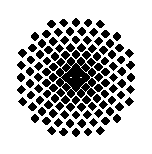
\includegraphics[width=20mm]{university-logo}
	\hspace{6mm}
	\ifthenelse{\equal{\doclang}{german}}{
		\begin{minipage}[b]{.6\textwidth}
			{\Large Universit\"at Stuttgart } \\
			Institut f\"ur Signalverarbeitung und Systemtheorie\\
			Professor Dr.-Ing. B. Yang \vspace{0pt}
		\end{minipage}
	}{
		\begin{minipage}[b]{.6\textwidth}
			{\Large University of Stuttgart } \\
			Institute for Signal Processing and System Theory\\
			Professor Dr.-Ing. B. Yang \vspace{0pt}
		\end{minipage}
	}
	\hspace{1mm}
	
\includegraphics[width=28mm]{isslogocolor}
}
\subject{\worksubject\vspace*{-5mm}} % Art und Nummer der Arbeit
\title{\Large{\langtitle}}
\author{
	\large
	\ifthenelse{\equal{\doclang}{german}}{
		\begin{tabular}{rp{7cm}}
			\Large 
			Autor:      & \Large \student \vspace*{2mm}\\
			%    Matr.-Nr.:  & \studentID \\
			Ausgabe:    & \startdate \\
			Abgabe:     & \submission \vspace*{3mm}\\
			Betreuer:   & \tutor \vspace*{2mm}\\
			Stichworte: & \keywords
		\end{tabular}
	}{
		\begin{tabular}{rp{7cm}}
			\Large 
			Authors:             & \Large \student \vspace*{2mm}\\
			%    Matr.-Nr.:          & \studentID \\
			Date of work begin: & \startdate \\
			Date of submission: & \submission \vspace*{3mm}\\
			Supervisor:         & \tutor \vspace*{2mm}\\
			Keywords:           & \keywords
		\end{tabular}
	}
	\bugfix
}
\date{}
\publishers{\normalsize
	\cleardoublepage
	\begin{minipage}[t]{.9\textwidth}
		\section*{Abstract}{%
		\enabstract}
	\end{minipage}	
	\begin{minipage}[t]{.9\textwidth}
		\section*{Kurzfassung}{%
		\deabstract}
	\end{minipage}
}

\numberwithin{equation}{chapter} 
\sloppy 

%
%
%
% *****************************************************************
% --------------> put typography definitions here <----------------
% *****************************************************************
% colors
\definecolor{darkblue}{rgb}{0,0,0.4}

% declarations
\newcommand{\matlab}{\textsc{Matlab}\raisebox{1ex}{\tiny{\textregistered}} }
\newcommand{\Z}{\mathbb{Z}}
\newcommand{\N}{\mathbb{N}}
\newcommand{\R}{\mathbb{R}}
\newcommand{\E}{\operatorname{E}}
\newcommand{\e}[1]{\operatorname{e}^{\,#1}}
\newcommand{\op}[1]{\operatorname{#1}}
\newcommand{\smtext}[1]{{\scriptscriptstyle\text{#1}}}

% unknown hyphenation rules
\hyphenation{Im-puls-ant-wort Im-puls-ant-wort-ko-ef-fi-zien-ten
	Pro-gramm-aus-schnitt Mi-kro-fon-sig-nal}
% *****************************************************************
%
%
%
% *****************************************************************
\begin{document}
	
	% title and table of contents
	\pagenumbering{Roman} % roman numbering for table of contents
	\maketitle
	\tableofcontents
	\cleardoublepage
	\setcounter{page}{1}
	\pagenumbering{arabic} % arabic numbering for rest of document
	
	% *****************************************************************
	% -------------------> start writing here <------------------------
\chapter{Introduction}
The field of unsupervised learning is fundamental in machine learning. Since nearly every novel product is connected, a tremendous amount of data is generated. Labelling all the data is not feasible and to save it is neither possible nor desired, since in most applications not all recorded date is useful. Therefore, in the area of unsupervised learning, tasks like dimensionality reduction (sometimes also called representation learning) or clustering are important to extract relevant features or/and group similar data together. Those two tasks are directly linked, since state-of-the-art clustering methods use as first step a dimensionality reduction to reduce the feature space and extract the relevant features out of the original data. Nevertheless, these models are usually build in an encoding/decoding scheme, so they not just focus on the dimensionality reduction but also on reconstructing the data out of the low-dimensional representation. The reduced feature space should be on the one hand a good representation in terms of clustering similar data, but on the other hand allow a good reconstruction of the original data. Those two tasks can be contrary to each other, e.g. when for a good reconstruction in pixel space the background colour of the image is important, but this is not relevant for detecting and clustering similar objects in the feature space. An example are pictures of a flying bird and a flying air plane. Both fly in the sky, that's why images of these two categories will in the most cases contain many blue pixels due to the sky in the background  but just a few other pixels that make the distinction. For reconstruction in pixel space the encoding of (for clustering) potentially unnecessary but space consuming information such as the sky could be favoured. In literature this problem is often called blue-sky problem \cite{Haeusser18bluesky}.\\
In most of the works a deep auto-encoder (or a variation of it) is first trained to extract the relevant features but also ensure a good reconstruction of the latent space. Different learning approaches exist to achieve this task. Traditionally, most learning approaches treat feature-selection/representation-learning and clustering separately. However, some new approaches outperform traditional ones, by combining these two task. In this work, both options are represented. Although in all of those works a very good performance (in this case clustering accuracy) and generalizability is claimed, the experiments given in the publications are often limited with respect to datasets and/or variation of hyperparameters. Therefore, in this work, different methods for clustering images are implemented and evaluated inside a framework, which is developed in this work within Tensorflow, to allow a fair comparison of those methods.\\
First, a short overview of the theoretical background for deep learning and unsupervised learning will be given, followed by a more specific part about the idea and main algorithms for dimensionality reduction/ representation learning and clustering. Chapter two will explain the working environment which will be further used in this work. The third chapter introduces the used architectures and algorithms, as well as the related hyperparameters of the models. The mentioned algorithms are implemented inside the environment explained in chapter two. Chapter four defines the experimental setup for the evaluation of the models. Further the used datasets as well as the investigated hyperparameters are introduced. Following this chapter, the results of the experiments are discussed and visualized in chapter five. The final chapter six summarizes the work and gives a outlook about further possible investigations or steps which can be derived based on this work.

\chapter{Theoretical background}
This chapter gives a short overview about the theoretical basics which are necessary for the following work. First, a general overview about deep learning is given with respect to its main critical parts. Then a more detailed part about unsupervised learning followed by more specific ones about dimensionality reduction and clustering. General it can be said that dimensionality reduction and clustering are specific tasks of unsupervised learning, which is a sub domain of deep learning. A graphical overview of the relationship between the mentioned domains is given in figure \ref{fig:Relationship_DL}. 
\begin{figure}[htb!]
	\centering
	\includegraphics[width=0.5\linewidth]{Graphiken/Overview_Deep_Learning}
	\caption{Relationship between deep learning, unsupervised learning, clustering and dimensionality reduction}
	\label{fig:Relationship_DL}
\end{figure}
The following section will give a rough overview about deep learning, the way deep neural networks actually work and how it is possible to train them. First, the relation between deep learning and machine learning is explained. Then the general structure and behaviour of a neural network is explained and the algorithm for training those networks is introduced. Finally some difficulties in training these networks are named with corresponding solutions. Due to focussing on the main part of the research thesis, the basics of the mentioned points are introduced, but not every thing is discussed and explained in detail. For more detailed explanations, please refer to the corresponding references.\\
\section{Deep Learning}
Deep learning is a sub area of machine learning, which is in general a learning-based or data-driven approach to design a processing rule (see figure \ref{fig:ProcessingRule}). The learning of this processing rule is based on examples. So it's obvious that the choice of training samples is crucial for learning a good and generalized processing rule. 
\begin{figure}[htb!]
	\centering
	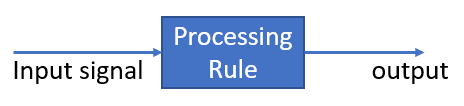
\includegraphics[width=0.5\linewidth]{Graphiken/ProcessingRule}
	\caption{General problem formulation in machine learning}
	\label{fig:ProcessingRule}
\end{figure}
There is one main difference between conventional machine learning and deep learning. While they have in common, that they get input data which is preprocessed depending on the application, in conventional machine learning features are extracted based on a defined rule \cite{Goodfellow-et-al-2016}. For this task, no theory exists and experience is necessary to choose good and relevant features for the following task, e.g. classification. The classification is done by a classifier, like kNN (k-nearest neighbour) or SVM (Support Vector Machine). In deep learning, there exists just one so-called deep neural network (DNN) for the tasks feature extraction and classification. The DNN learns and adapts the network parameters by a proper loss function. This can be obtained efficiently using the technique of (error) backpropagation (\cite{Goodfellow-et-al-2016}, \cite{Nielsen-Michael}, \cite{DeepLearningDive}, \cite{Bishop}). More details will be given in the following.\\
The learning strategy for DNNs is adapted from the way humans learn to recognize, speak, walk, calculate etc.. Despite deep learning is often seen as a exciting new technology, it can be dated back to the 1940s. Following \cite{Goodfellow-et-al-2016}, there have been three waves of development: In the 1940s-1960s (known as cybernetics), between 1980 and 1990 as connectionism and the current resurgence under the recent name deep learning beginning in 2006. The third wave of development, which is still in progress began with a breakthrough by Geoffrey Hinton. He showed that a special kind of neural network, the so called "Deep Belief Network" could be trained efficiently using a strategy called greedy layer-wise pretraining \cite{Hinton-et-al-2006}.\\
Since this breakthrough, the applications of deep neural networks increase tremendously. Examples for applications of deep neural networks nowadays are recommender systems, automatic speech recognition, text to speech translation, image recognition and/or segmentation and a lot more \cite{DeepLearningDive}. For a special task the networks are typically adjusted and the architecture is adapted. Therefore a lot of variation of deep neural networks exists nowadays, examples mentioned in \cite{Nielsen-Michael} are convolutional neural networks (CNNs), recurrent neural networks (RNNs) or deep belief nets (DBNs).\\
In the following, the architecture of a feedforward neural network is shown exemplary, since the deep feedforward networks, also often called feedforward neural networks or multilayer perceptrons (MLPs), are the basic deep learning models \cite{Goodfellow-et-al-2016}. The naming \textit{feedforward} comes from property, that information flows in forward direction through the network, so from the input signal to the output. There is no feedback connection inside the model. These feedforward neural networks consists of multiple layers stacked together to a network. Each layer consists of many neurons. Figure \ref{fig:SingleNeuron} shows one single neuron.
\begin{figure}[htb!]
	\centering
	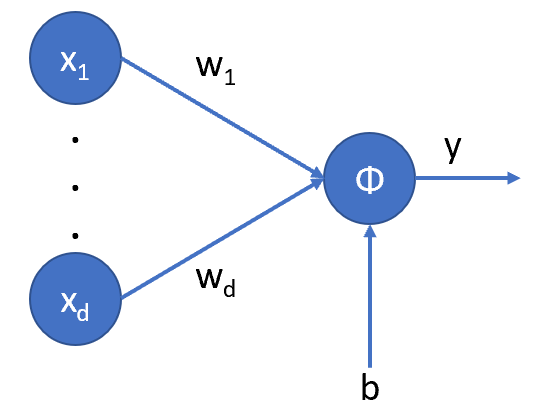
\includegraphics[width=0.3\linewidth]{Graphiken/SingleNeuron}
	\caption{Single Neuron in a feedforward neural network}
	\label{fig:SingleNeuron}
\end{figure}
In equation \ref{eq:singleneuron}, the output $y$ of a single neuron is given, with $\phi$ is the (typically non-linear) activation function of the activation $a$ which is an affine function in $\underline{x}$. $\underline{x}$ is the input, which can be a vector, a 2-d image or a 3-d tensor. The trainable parameters of the neuron are the weights $\underline{w}$ and the bias $b$.
\begin{align}
	a = \underline{w}{^T}\underline{x}+b\\
	y = \phi(a) \label{eq:singleneuron}
\end{align}
A layer of neurons, as drawn in figure \ref{fig:Layer_of_neurons}, consists of $c$ neurons, which are connected with the input and output. The neurons in the same layer are not interconnected between each other. Depending on the network structure, the connections to the input and output varies. Two of the most popular layer structures are dense (or fully connected) and convolutional layer. For a dense (or fully connected) layer, each input $x_{j}$ is connected to each neuron $i$. The drawbacks of fully connected networks (FCN - network consisting of just fully connected layers) are the huge number of parameters, so a tremendous computational and memory complexity is the result. As a consequence of its connection schema, it does not learn local patterns/features of input signals since all neurons are fully connected. This problems can be solved by using a convolutional neural network (CNN - network consisting mainly of convolutional layers). Due to the properties of sparse connections and parameter sharing, the memory complexity is reduced and the networks is able to recognize input pattern regardless of its position, so a CNN focusses on local input patterns \cite{LectureNotes_DeepLearning}.
\begin{figure}[htb!]
	\centering
	\subfloat[Layer of Neurons\label{fig:NeuronsLayer}]{%			
		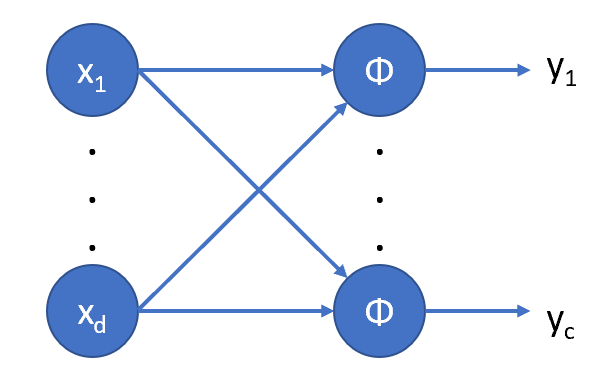
\includegraphics[width=0.45\linewidth]{Graphiken/NeuronsLayer}}
	\qquad
	\subfloat[Layer of Neurons compressed visualization\label{fig:NeuronsLayer_Matrix}]{%			
		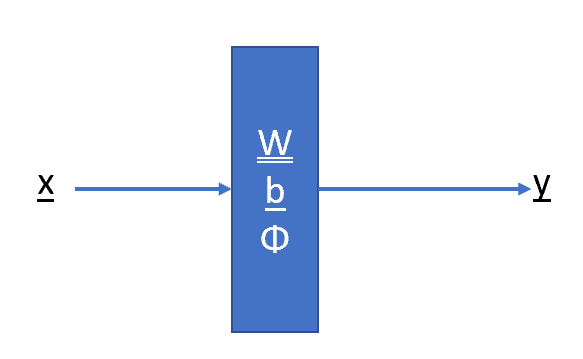
\includegraphics[width=0.45\linewidth]{Graphiken/NeuronsLayer_Matrix}}
	\caption{Layer of Neurons in feedforward neural network}
	\label{fig:Layer_of_neurons}
\end{figure}
After defining one layer, a layer can be stacked to another one and so on. By stacking single layers together, the resulting architecture is denoted as a neural network. The overall length of the chain gives the depth of the model. From this terminology, the name deep learning arose. The first layer of a network is called the \textit{input layer}, while the last one is correspondingly named \textit{output layer}. Those two layers have fixed sizes, since the input and the output data of a network has a defined size. All layers between them are called hidden layers. These layers are called hidden since they are neither visible to the inputs nor the outputs. Different to the the input and output layers, their size is not fixed. They are generally used to form a \textit{bottleneck}, forcing the network to make a simple model of the system with the ability to generalise to previously unseen patterns (test data) \cite{Michie-et-al-1994}. By using non-linear activation functions, such as softmax (equation \ref{eq:softmax}) or rectifier linear unit (ReLU) (equation \ref{eq:ReLU}), it can be shown that already a simple two-layer MLP can approximate an arbitrary continuous mapping arbitrarily closely if there the number of hidden nodes is not limited \cite{Michie-et-al-1994}. This property of neural networks is also known as universal function approximation.
\begin{align}
	\phi_{i}(\underline{a}) = \frac{e^{a_{i}}}{\sum_{j=1}^{c}e^{a_{j}}} \label{eq:softmax}\\
	\phi_{i}(a_{i}) = \begin{cases} a_i & a_{i} > 0\\0 & a_{i} \leq 0\\ \end{cases} \label{eq:ReLU}
\end{align}
If linear activation functions would be used, the overall network, independent on the depth of the network, will overall be just a linear transformation of the input data, so only linear solvable problems could be solved. This shows the importance for choosing non-linear activation functions.\\
To train a neural network regarding the desired behaviour, a proper loss function based on the training data has to be defined, which has to be minimized with respect to the network parameters. 
In general, the training objective of a neural network is to minimize the cost function $L(\underline{\theta})$ on the training data as given in equation \ref{eq:CostFunction} with $\iota(\underline{x}(n),\underline{y}(n);\underline{\theta})$ is an arbitrary loss function where $\underline{y}$ is the target output of the network and $\underline{x}$ is the input of the network. The cost function denotes the total loss over all $N$ samples.
\begin{align}
	\underset{\underline{\theta}}\min L(\underline{\theta}) = \frac{1}{N}\sum_{n=1}^{N}\iota(\underline{x}(n),\underline{y}(n);\underline{\theta})  \label{eq:CostFunction}
\end{align}
The loss function is depending on the task. For regression, a typical loss function is the $l_{2}$-loss, where $l_{2}$-Norm of the error is used. The error is the difference between the target output $\underline{y}$ and the output of the neural network, $f(\underline{x};\underline{\theta})$. This loss function is given in equation \ref{eq:l2-loss}.
\begin{align}
	\iota(\underline{x},\underline{y};\underline{\theta}) = ||\underline{y}-f(\underline{x};\underline{\theta})||^{2}\label{eq:l2-loss}
\end{align}
For classification, a typical loss function is the categorical loss. Equation \ref{eq:cat-loss} denotes this loss function.
\begin{align}
	\iota(\underline{x},\underline{y};\underline{\theta}) = -\underline{y}^{T}ln f(\underline{x};\underline{\theta})\label{eq:cat-loss}
\end{align}
The target is to find $\underset{\underline{\theta}}\min L(\underline{\theta})$, which has in general no closed-form solution. Therefore, numerical optimization is used in deep learning. The standard algorithm for minimizing the loss function in deep learning is the gradient descent (GD) algorithm. In this algorithm, the gradient information is used to choose the parameter update to perform a small step in the direction of the negative gradient \cite{Bishop}. Equation \ref{eq:GradientDescent_update} formulates the update step of the GD-algorithm where $t \in \mathbb{Z}_{\geq0}$ is the iteration index and $\eta > 0$ is the step size or learning rate. $\underline{\theta}^{0}$ is the initialization of the network and an initial guess for $\underline{\theta}$.
\begin{align}
	\underline{\theta}^{t+1} = \underline{\theta}^{t} - \eta\underline{\nabla}L(\underline{\theta})|_{\underline{\theta}=\underline{\theta}^{t}}\label{eq:GradientDescent_update}
\end{align}
Due to the size of the training datasets (e.g. 55000 images for MNIST), not the whole dataset can be kept in the memory. Therefore stochastic gradient descent is used to reduce the computing cost for each iteration, where the gradient vector $\underline{\nabla}L$ and the update $\underline{\theta}^{t+1}$ is calculated for one minibatch $i$. The stochastic gradient $\underline{\nabla}L_{i}$ is the unbiased estimate of the gradient $\underline{\nabla}L$, resulting in a more noisy gradient which lead to the name \textbf{stochastic} gradient descent \cite{DeepLearningDive}.\\
It is obvious, that the calculation of $\underline{\nabla}L$ is crucial for performing an update step. Therefore, the partial derivatives of the cost function with respect to the network parameters $w$ and $b$ have to be calculated: $\dfrac{\partial L}{\partial w}$ and $\dfrac{\partial L}{\partial b}$. This can be done efficiently by using the error backpropagation algorithm (sometimes just called \textit{backpropagation} or \textit{backprop}). As the name denotes, the error vectors are backpropagated through the network. Starting at the output layer $L$, the  error vector of this layer with respect to the weights $w_{L_{ij}}$ is given in equation \ref{eq:ErrorVector_OutputLayer} with $\underline{x}_{L}$ as the output and $\underline{a}_{L}$ as activation of layer $L$. Calculating the partial derivative with respect to $b$ follows the same formulas.
\begin{align}
	\underline{\delta}_{L}^{T} = \dfrac{\partial L(\underline{\theta})}{\partial w_{L_{ij}}} = \dfrac{\partial L}{\partial \underline{x}_{L}}\dfrac{\partial \underline{x}_{L}}{\partial \underline{a}_{L}}\dfrac{\partial \underline{a}_{L}}{\partial w_{L_{ij}}}\label{eq:ErrorVector_OutputLayer}
\end{align}
For the remaining layers $l \in [1, L-1]$ the error vector can be calculated by applying the chain rule for differentiation. The error vector for layer $l$ can be calculated with equation \ref{eq:ErrorVector_generalLayer} \cite{LectureNotes_DeepLearning}.
\begin{align}
	\underline{\delta}_{l}^{T} = \underline{\delta}_{l+1}^{T}\dfrac{\partial \underline{a}_{l+1}}{\partial a_{l}}\dfrac{\partial \underline{a}_{l}}{\partial w_{l_{ij}}}\label{eq:ErrorVector_generalLayer}
\end{align}
Figure \ref{fig:Backprop_DNN} gives a graphical representation of the paths through a DNN. Figure \ref{fig:ForwardPass_DNN} shows the forward path through a DNN for calculating the cost values. Figure \ref{fig:BackwardPass_DNN} shows the backpropagation of the error vectors through the network.
\begin{figure}[htb!]
	\centering
	\subfloat[Forward path through a network\label{fig:ForwardPass_DNN}]{%			
		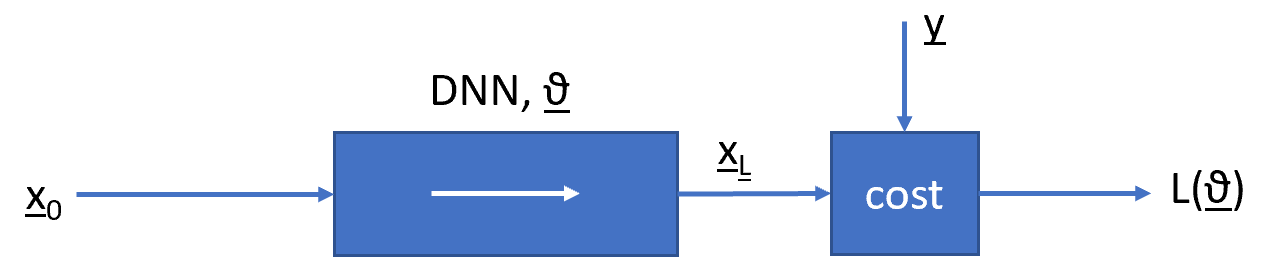
\includegraphics[width=0.5\linewidth]{Graphiken/ForwardPass_DNN}}
	\qquad
	\subfloat[Error Backpropagation\label{fig:BackwardPass_DNN}]{%			
		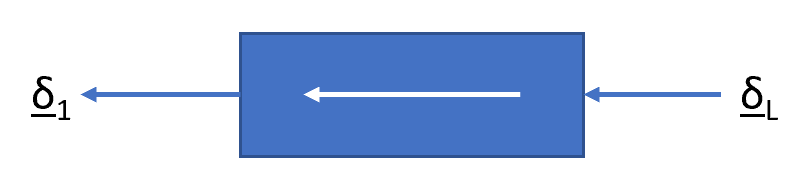
\includegraphics[width=0.3\linewidth]{Graphiken/BackwardPass_DNN}}
	\caption{Forward path and backpropagation through a neural network}
	\label{fig:Backprop_DNN}
\end{figure}
By backpropagating through the network, $\underline{\delta}_{1}^{T}$ gives in the end the error vector of the network. This information will then be used to update the weights and biases following an numerical optimization algorithm like the stochastic gradient descent algorithm.\\
\cite{Bishop} summarizes the error backpropagation in four steps:
\begin{enumerate}
	\item Apply the input $\underline{x}_{0}$ to the network and forward propagate through the network as in figure \ref{fig:ForwardPass_DNN} to find activations of all the hidden and output units.
	\item Evaluate the error vector $\underline{\delta}_{L}^{T}$ for all output units using equation \ref{eq:ErrorVector_OutputLayer}
	\item Backpropagate the error vectors through $\underline{\delta}_{l}^{T}$ the network following \ref{eq:ErrorVector_generalLayer} to obtain the error vector for each hidden unit in the network (figure \ref{fig:BackwardPass_DNN})
	\item Apply a numerical optimization algorithm (i.e. SGD) to adapt the network parameters
\end{enumerate}
Training (optimizing) a neural network is a difficult task and suffers from a number of optimization difficulties. Table \ref{tab:Difficulties} gives a rough summary about the difficulties in optimizing a neural network and possible solutions\cite{LectureNotes_DeepLearning}.\\
\begin{table}
    \centering
    \caption{Difficulties in optimizing a neural network}
    \label{tab:Difficulties}
    \begin{tabular}{lcc}
        \toprule
        Difficulty & Solutions\\
        \midrule
        stochastic gradient & larger minibatch size, momentum\\
        ill conditioning & momentum, input scaling and batch normalization\\
        saddle point / plateau & noisy gradient\\
        sensitive to step size & learning rate schedule\\
        local minimum & parameter initialization\\
        vanishing gradient & parameter initialization, improved model\\
        \bottomrule
    \end{tabular}
\end{table}
As mentioned in \cite{DeepLearningDive}, optimization provides a way to minimize the loss function for deep learning, but, in essence, the goals of optimization and deep learning are different. In pure optimization, the target is to minimize the (training) loss function. But in deep learning, the focus lies on minimizing the generalization error, which is the value of the loss function computed on new, unseen data (test data). Thus it is important to regularly apply test data to the network while training, to see if the network is overfitted to the training data. This means, the error on the training data is very small in comparison to the test/generalization error. There are various methods to ensure overfitting does not take place, i.e. dropout or regularization (\cite{Goodfellow-et-al-2016}, \cite{Nielsen-Michael}, \cite{DeepLearningDive}, \cite{Bishop}).\\
\section{Unsupervised Learning}
This section will give an overview of unsupervised learning and will give more details about two main tasks of unsupervised learning: dimensionality reduction/representation learning and clustering.\\
Unsupervised learning offers the possibility of exploring structure of data without guidance in the form of class information, which leads to the name \textit{unsupervised}. In comparison to supervised or semi-supervised learning, no class information (i.e. no class labels) are available while training. This can  reveal features not previously expected or known about \cite{Michie-et-al-1994}.\\
In the task dimensionality reduction or representation learning, the task is to find a representation of the original data in a lower dimensional feature space. So it offers a model of the data in fewer parameters than were required to store the entire training data in the original format. This has big advantages for storing, coding and transmitting data. After learning the hidden representations by an encoding and decoding form, some models are able to generate new data with same characteristic as the original data when required. These models are called generative models.\\
When having datasets without labels, in most applications it is relevant to cluster similar data points together. Therefore clustering can be applied. Intuitively, it is assumed that inter-points similarities are high in a group of data points which belong to the same cluster and vice-versa. The similarity measure could be any kind of measure, i.e. euclidean distance or a probability value (probability belonging to a cluster). Popular clustering techniques are K-means clustering \cite{Lloyd82leastsquares}, DBSCAN \cite{Ester96adensity-based} or Gaussian Mixture Model (GMM) \cite{Gilles07MixtureModelsforClassification}. In Image segmentation, the original image has already a high dimensional. Even relatively small images, e.g. 32x32x1 images, have a 1024-dimensional feature space. In a high-dimensional feature space, similarity measures as euclidean distance are getting weaker to find similarities, also known as the course of dimensionality (first introduced by \cite{Bellman34}). Due to this, and the idea of clustering data based on relevant extracted features, the state-of-the-art for clustering is not using the original data, but extract relevant features by applying dimensionality reduction/representation learning to the data, and use a clustering algorithm on the \textit{bottleneck} representation of the data (the so called latent space).
\subsection{Dimensionality Reduction/Representation Learning}
As mentioned above, the idea is to reduce the dimensionality of the original data but still have meaningful representations of it. Generally, a good representation of the data is desired, which is one that makes a subsequent learning task easier \cite{Goodfellow-et-al-2016}. In the objective of this work, the subsequent learning task is clustering. In this work, autoencoder models and variations of it are used for the task of dimensionality reduction. Figure \ref{fig:Autoencoder} illustrates the general architecture of an autoencoder with an input $\underline{x}$, the latent representation $\underline{z}$ of the data and the reconstruction $\underline{\hat{y}}$. As ground truth for the loss calculation the original input is used and compared to the reconstructed one. This loss is called the reconstruction loss $L_{r}$.
\begin{figure}[htb!]
	\centering
	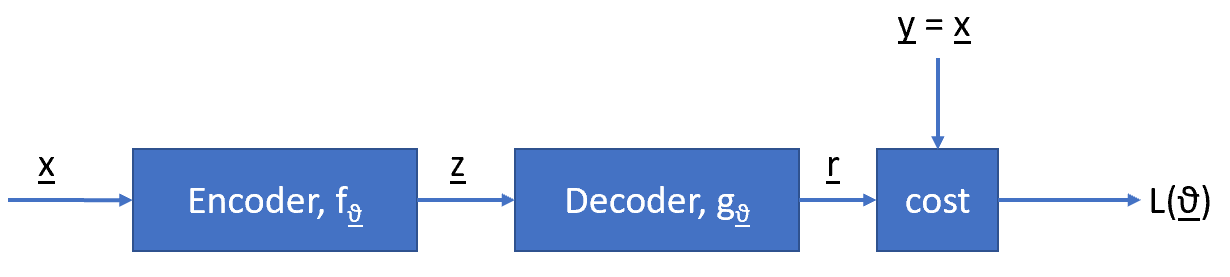
\includegraphics[width=0.6\linewidth]{Graphiken/Autoencoder_Architecture}
	\caption{General architecture of an autoencoder}
	\label{fig:Autoencoder}
\end{figure}
As seen in figure \ref{fig:Autoencoder}, the autoencoder consists of two parts, the encoder and decoder. The encoder can be seen as feature-extracting function $f_{\underline{\theta}}$ which will allow a straightforward and efficient computation of a feature vector $\underline{z} = f_{\underline{\theta}}(\underline{x})$ from an input $\underline{x}$. For each sample $\underline{x}(n), n \in [1,N]$ $\underline{z}(n)$ is defined as feature-vector/representation/code/embedding or latent variable from $\underline{x}(n)$ (see equation \ref{eq:Embedding_z}). 
\begin{align}
	\underline{z}(n) = f_{\underline{\theta}}(\underline{x}(n))\label{eq:Embedding_z}
\end{align}
The decoder function $g_{\underline{\theta}}$ maps from latent space back into the original input space producing the so-called reconstruction $\underline{r}$, which is defined in equation \ref{eq:Reconstruction}.
\begin{align}
	\underline{r} = g_{\underline{\theta}}(\underline{z}) = g_{\underline{\theta}}(f_{\underline{\theta}}(\underline{x}(n)))\label{eq:Reconstruction}
\end{align}
The set of parameters $\underline{\theta}$ of the encoder and decoder are learned simultaneously on the task of reconstructing the original input as well as possible, minimizing the reconstruction loss $L_{r}(\underline{x},\underline{r})$.\\
Mostly (also in this work), undercomplete or regularized autoencoders are used. These architectures ensure a dimensionality reduction by using a bottleneck, i.e. $d_{\underline{z}} << d_{\underline{x}}$. This clearly achieves a dimensionality reduction, but it is also helpful in terms of overfitting. When $d_{\underline{z}} \geq d_{\underline{x}}$, this can allow the autoencoder to simply duplicate the input in the features, thus achieving (nearly) perfect reconstruction without having extracted more meaningful features \cite{Bengio-et-al-2013}.\\
In this work, the focus is on achieving meaningful latent representations $\underline{z}$ since these latent representations will further be used as input for the clustering step. More details about the detailed architecture of the dimensionality reduction/representation learning part of the model will be discussed in the corresponding sections.
\subsection{Clustering algorithm}
The main objective of clustering is to separate data into groups of similar data points. Clustering algorithms should, in principal, be able to answer two questions:
\begin{enumerate}
	\item Which samples belongs to the same cluster?
	\item How man clusters exist in the dataset?
\end{enumerate}
Based on these questions, it can be split between two groups of clustering algorithms. The first one can't answer question 2. They need a-priori information about the number of clusters in the dataset. Examples for this group of algorithms are K-means \cite{Lloyd82leastsquares}, fuzzy c-means \cite{Bezdek81fuzzycmenas} or Gaussian Mixture Model (GMM) \cite{Gilles07MixtureModelsforClassification}.\\
The second group does not need this information, these algorithms are constructed to find the number of clusters while the clustering process by itself. Examples for this kind of algorithms are DBSCAN \cite{Ester96adensity-based} or mean-shift clustering \cite{Fukunaga75mean-shift}.\\
In this work, the clustering algorithm K-means is used, since it is the typically used algorithm for the clustering step in state-of-the-art clustering models. The K-means algorithm will be explained in more detail in the following.
\subsubsection{K-means Clustering}
As already described, the problem of clustering is identifying groups (clusters) of data points in a d-dimensional space. Given the number of clusters as $K$, big inter-samples similarities within a cluster compared to the samples of another cluster are desired. To measure the similarity from a sample to a cluster, a cluster representation, the cluster center $\underline{\mu}_{k}$ for each cluster, is defined. Following this, the samples are assigned to the clusters, which will be done by assigning each sample to the cluster with the nearest center (nearest-mean assignment). This is expressed by a binary indicator variable $r_{nk}$, with $r_{nk} = 1$ if the sample $\underline{x}_{n}$ is assigned to cluster $k$ and $r_{nk} = 0$ otherwise. With these definitions, an objective function can be defined, given in equation \ref{eq:kMeans_Objective} with $sim(\underline{x}_{n}, \underline{\mu}_{k})$ can be any similarity or dissimilarity metric (i.e. euclidean distance or cosine similarity).
\begin{align}
J = \sum_{n=1}^{N} \sum_{k=1}^{K} r_{nk} sim(\underline{x}_{n}, \underline{\mu}_{k})\label{eq:kMeans_Objective}
\end{align}
As an example, the squared euclidean distance is chosen as dissimilarity metric (equation \ref{eq:squared_euclidean_distance}).
\begin{align}
sim(\underline{x}_{n}, \underline{\mu}_{k}) = ||\underline{x}_{n} - \underline{\mu}_{k}||^{2}\label{eq:squared_euclidean_distance}
\end{align}
Having a measure for the similarity, the cluster assignment can be defined as following (equation):
\begin{align}
r_{nk} = \begin{cases} 1 & if\ k = arg\ \underset{j}\min ||\underline{x}_{n} - \underline{\mu}_{j}||^{2}\\0 & otherwise\end{cases}\label{eq:sample_clusterassignment}
\end{align}
Using the defined formulas, the goal is to find the values of $r_{nk}$ and $\underline{\mu}_{k}$ which minimize $J$. This can be done by an iterative procedure where every iteration contains of two steps. First fix $\underline{\mu}_{k}$ and assign the samples to the cluster centers, so update $r_{nk}$ to minimize J. In the second step fix $r_{nk}$ and update $\underline{\mu}_{k}$. This can be done for a defined number of iterations or until convergence (no change in cluster assignments) \cite{Bishop}.\\
The algorithm is summarized in the following \cite{LectureNotes_DPR}:
\begin{algorithm}
\caption{K-Means training algorithm}
\begin{algorithmic}
\Inputs{samples $S=\lbrace\underline{x}_1,...,\underline{x}:N\rbrace$}
\Initialize{Initialization of cluster centers \\ $i=0$}
\While{$i \leq max\_iter$ or change in clusters $S_i$}
\State Cluster $S_i, 1 \leq i \leq k \gets$ Assign each $\underline{x}_n$ to nearest cluster $j$ (with mean $\underline{\mu}_j$)
\State recompute the cluster centers (equation \ref{eq:cluster_center_update}) 
\begin{align} 
\underline{\mu}_{j} = \dfrac{1}{|S_{i}|} \sum_{\underline{x}_{n} \in S_{i}}\underline{x}_{n}\label{eq:cluster_center_update}
\end{align}
\State $i \gets i+1$
\EndWhile
\end{algorithmic}
\end{algorithm}
It is obvious, that the convergence time of the algorithm is sensitive to the choice of the initial cluster centers. An naive (and fast) approach is to randomly choose samples out of $S$ to initialize the cluster centers. Nevertheless, there are more improved initialization schemes available (\cite{Yi10ImprovedInitialization}, \cite{Arthuer07kmeans_plusplus}). In this work the Tensorflow built-in minibatch algorithm of K-means is used, due to limited memory and the sizes of the datasets. As initialization the built-in \textit{K-means plus plus} functionality is used.
\chapter{Working Environment (Framework)}
In this chapter the working environment for evaluating the models is introduced. First, the software environment, namely TensorFlow, is introduced shortly. Secondly, the framework, which was developed in this work, is introduced.
\paragraph{TensorFlow}\mbox{}\\
TensorFlow is an interface to express machine learning algorithms and an implementation to execute such algorithms. It is a system that was developed to operate at large scale and in heterogeneous environments. The focus of TensorFlow is on training and inference on deep neural networks. It uses dataflow graphs to represent computation, shared state and the operations \cite{tensorflow2015-whitepaper}. In this work, the TensorFlow Version 1.13 is used.
\paragraph{Framework}\mbox{}\\
The implemented framework is used to have an easy comparison of different models, i.e. in using the same training procedure and same evaluation metrics. Therefore, the implementation has to be as modular as possible, so that new architectures could easily be implemented and evaluated. But on the other side, clear interfaces are defined for every model so that a general training algorithm can be used which allows comparability. The program flow is as following:
\begin{enumerate}
	\item Parameters are set in a separate parameter file
	\item The inputs for the models are defined. Separate inputs are created for the training and clustering part. An iterator with the desired attributes (i.e. batch-size, shuffling, image resizing, data augmentation) is returned 
	\item The \textit{train model} is created, which is the model to extract features out of the original data. The \textit{train model spec} is returned containing the necessary operations (i.e. initialization, optimization, metric updates etc.) and the interface to the latent representation for clustering
	\item The \textit{cluster model} is created, which is the model to cluster the data based on the latent representation of the \textit{train model}. The \textit{cluster model spec} is returned containing the necessary operations (i.e. initialization, cluster adjustments, cluster assignments, metric updates etc.).
	\item The created models are transmitted to a function for training and evaluation. This training and evaluation step is repeated until the defined number of epochs is reached.
		\begin{description}
			\item[Training:] Execute the training operation of the \textit{train model} for one iteration over the whole training data, update the defined metrics and write them to the Tensorboard
			\item[Evaluation:] The clustering is executed on all clustering data and the corresponding metrics are calculated and written to Tensorboard. If selected, the latent space is visualized in a 2-dimensional space with the help of UMAP \cite{mcinnes2018umap-software} and t-SNE \cite{t-SNE}.			
		\end{description}
\end{enumerate}
The desired dataset, feature extraction model and clustering algorithm is selected when executing the program by argument parsers. Based on the selected combination and time, the summaries from training and evaluation are stored in a folder with unique naming. Also the parameters are stored there, so the results can be reproduced easily. The implemented models will be introduced in the next chapter.
\chapter{Model Architectures and Algorithm}
In this chapter, the implemented and evaluated architectures and algorithms will be explained in detail. Therefore, the corresponding loss functions, the training procedure and also model-related hyperparameters are introduced. The most parts are models for representation learning and thus used as feature extractor. They base on autoencoder structure, but differ all slightly . Also, one additional clustering algorithm (in addition to the already introduced K-means clustering algorithm), the Improved Deep Embedding Clustering (IDEC) algorithm, is introduced.
\section{Autoencoder}
\label{sec:AE}
The general architecture of an autoencoder (figure \ref{fig:Autoencoder}), the formulation for the latent space $\underline{z}(n)$ (formula \ref{eq:Embedding_z}) and the reconstruction $\underline{r}$ (formula \ref{eq:Reconstruction}) is already introduced. To achieve a meaningful latent representation, undercomplete autoencoder are used in this work to force the model to capture the most important features of the input data \cite{LectureNotes_DeepLearning}. Thus we have a bottleneck of a parametrized size $n\_latent$, so $\underline{z}(n) \in \mathbb{R}^{n\_latent}$. As \cite{Bengio-et-al-2013} states, one can view the objective of the regularization applied to an autoencoder as making the representation as constant (insensitive) as possible with respect to changes in input. For the clustering tasks, this means that i.e. when clustering dogs and cats, different kind of dogs should be mapped to a similar latent representation, so this latent representation should be as constant as possible for this cluster.\\
In this work, deep autoencoder models with convolutional and deconvoluational layers are used, a Deep Convolutional Autoencoder \cite{DeepCAE}. By this, it takes advantage of the properties of a convolutional neural network (CNN). The local connections and parameter sharing of a convolutional layer distinguish a CNN to have a property in translation latent features \cite{Goodfellow-et-al-2016}. Thus, by using a CNN-structure, a certain locality in feature calculation can be achieved, which means that only a small neighbourhood of pixels will be used for computation. This is a desirable property for images, since often the features (i.e. edges) are occurring in a certain neighbourhood. The encoder-decoder structure of the used autoencoder is given in figure \ref{fig:AE_ModelArchitecture} with example dimensions at each layer for an input image of size $32x32x1$.
\begin{figure}[htb!]
	\centering
	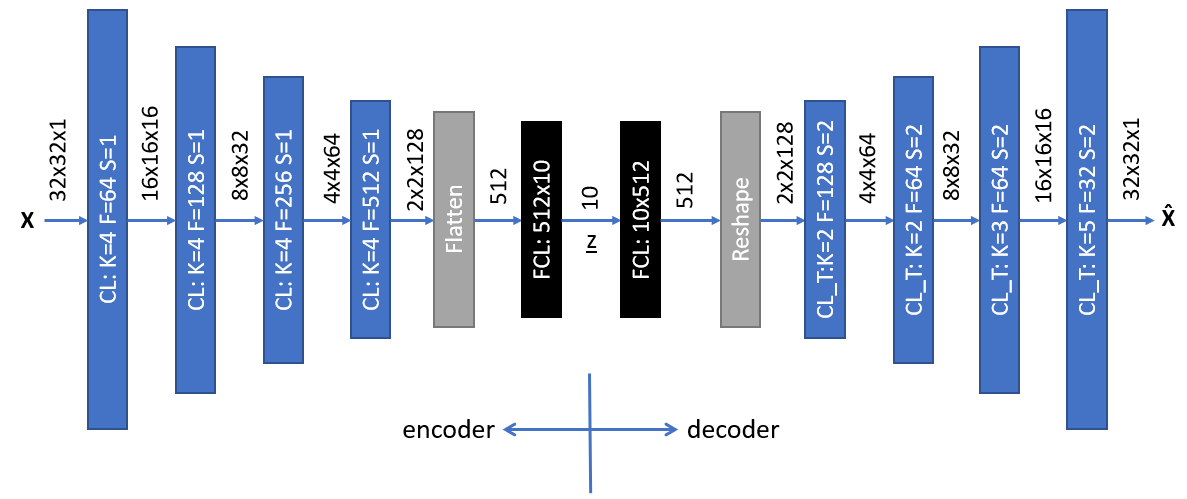
\includegraphics[width=0.9\linewidth]{Graphiken/Autoencoder_Model}
	\caption{Autoencoder Model Architecture}
	\label{fig:AE_ModelArchitecture}
\end{figure}
\textit{CL} is a convolutional layer with the kernel size \textit{K}, the filters \textit{F} and the Stride \textit{S}. The \textit{flatten}-layer flattens the input to a 1d-vector. FCL is a fully connected layer which here maps the input to the desired latent space size $n\_latent$, in the example this value is $10$. The decoder part is the mirrored encoder part with \textit{Reshape} reshapes the 1d-vector to its pervious size. \textit{CL\_T} are transposed convolutional layer with the same parameters as \textit{CL}. Transposed convolution is also known as \textit{fractionally-strided convolution} or \textit{deconvolution}. These layers are used to upsample the data by using a corresponding stride \cite{DeepLearningDive}. One convolutional layer $l$ is exemplary drawn in figure \ref{fig:Conv_layer}.
\begin{figure}[htb!]
	\centering
	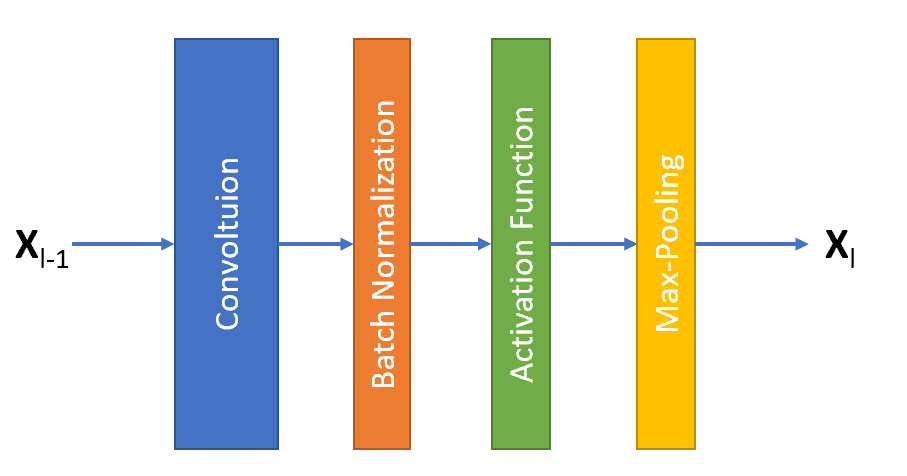
\includegraphics[width=0.5\linewidth]{Graphiken/ConvolutionalLayer}
	\caption{Covlutional Layer with its elements}
	\label{fig:Conv_layer}
\end{figure}
Each convolutional layer \textit{CL} of the model consists of several parts. They are listed and explained below.\\
\begin{description}
	\item[Convolution]\hfill \\
The 2-dimensional convolution takes place here. The input $\mathbf{X}_{l-1}$ of layer $l$ contains $D_{l-1}$ 2D feature maps of size $M_l\ x\ N_{l-1}			$. The convolution layer has $D_l$ kernels to calculate 2D feature maps of size $M_l\ x\ N_l$. Each kernel contains $D_{l-1}$ 2D filters of size $K_l\ 		x\ K_l$, each performing a sliding window convolution over the whole input.
	\item[Batch normalization]\hfill \\
Batch normalization, proposed by \cite{Ioffe15BatchNorm} in 2015, can be used to improve convergence of a deep neural network at training. Batch Normalization does a zero-mean unit-variance normalization for all elements of an activation $\underline{a}_l(n)$ for one minibatch $t$. It reduces the amount by what the hidden unit values shift around (known as covariance shift). As mentioned, the activations are approximately rescaled to zero-mean and unit-variance. Since this may not be desired, e.g. in some cases the activations need to differ from standardized data, some scaling coefficient $\gamma$ and an offset $\beta$ are introduced. The equation of Batch Normalization for one layer with input activation $\underline{a}_l$ is given in formula \ref{eq:batchnormalization} with the introduced parameters $\underline{\gamma}$ and $\underline{\beta}$. $\epsilon > 0$ is a small number (i.e. $10^{-5}$) to avoid division-by-zero. The calculations of the estimated mean $\underline{\hat{\mu}}_L$ and variance $\underline{\hat{\sigma}}_L$ for a minibatch $t$ at layer $l$ with  $N$ samples are given in formula \ref{eq:batchmean} and \ref{eq:batchvariance}.
\begin{align}
	BN(\underline{a}_l) = \underline{\gamma}_l\dfrac{\underline{a}_l-\underline{\hat{\mu}}_l}{\sqrt{\underline{\hat{\sigma}}_{l}^{2}+\epsilon}}+\underline{\beta}_l\label{eq:batchnormalization}\\
	\underline{\hat{\mu}}_l(t) = \dfrac{1}{N}\sum_{n=1}^{N}\underline{a}_l(n)\label{eq:batchmean}\\
	\underline{\hat{\sigma}}_{l}^{2}(t) = \dfrac{1}{N-1}\sum_{n=1}^{N}(\underline{a}_l(n)-\underline{\hat{\mu}}_l(t))^{2}\label{eq:batchvariance}
\end{align}		
The parameters $\underline{\gamma}$ and $\underline{\beta}$ are learned together with the network parameters $\theta$. This parametrization is easier to learn, since the offset and range of $\underline{a}_l$ is explicitly modelled by those parameters and is not determined by all previous layers in a hidden and complicated way. By normalizing the activation of a layer, the following layers can learn itself a little bit more independently of other layers. In addition, higher learning rates can be used because the batch normalization ensures that there's no activation that goes really high or really low (risk for vanishing/exploding gradient). Another property of batch normalization is the reducing of overfitting, because it has a slight regularization effect \cite{DeepLearningDive}, \cite{LectureNotes_DeepLearning}.
	\item[Leacky ReLU activation function]\hfill \\
	The leacky ReLU \cite{Xu15LReLU} is an activation out of the family of rectifier linear units (formula \ref{eq:ReLU}). These ReLU activation functions are currently one of the most popular in deep neural network architecture due to its low calculation complexity and differentiability. The leacky ReLU, as defined in equation \ref{eq:leackyReLU}, ensures a non-zero gradient for $ a < 0$ due to its factor $\xi >> 0$.
	\begin{align}
		\phi(a) = \begin{cases} a & a > 0\\ \dfrac{a}{\xi} & a \leq 0\\ \end{cases} \label{eq:leackyReLU}
	\end{align}	
	\item[Max-Pooling]\hfill \\
	A pooling function in general replaces the output of a layer at a certain location with a defined summary statistic of the nearby outputs. The size of nearby outputs is defined by a parameter. The pooling operations are used to get a certain degree of invariance to small translations. For instance, if an image $\mathbf{X}$ with a sharp boundary between white and black pixels is given, the output of the same image shifted one to the right, i.e. $\mathbf{Z}[i, j] = \mathbf{X}[i, j+1]$ will be vastly different if no pooling is used. The edge will be shifted by one pixels and with it all activations. Pooling would ensure the same activation as before in this case. Typical pooling functions are max-pooling and average pooling. These functions take the maximum (or average) in a defined neighbourhood of the pixel. It can be easily seen, that pooling reduces the size of the image by a factor, which is the multiplication of the neighbourhood sizes in the dimensions (\cite{Goodfellow-et-al-2016}, \cite{DeepLearningDive}). An example for max-pooling on a $4x4$ input image is given in figure \ref{fig:Max-Pooling}.
\begin{figure}[htb!]
	\centering
	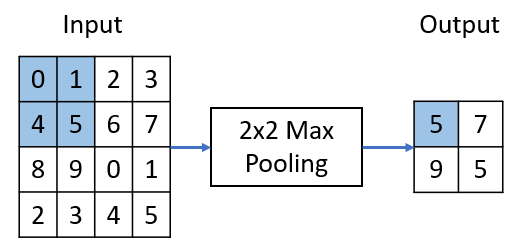
\includegraphics[width=0.5\linewidth]{Graphiken/2x2_MaxPooling}
	\caption{2x2 Max-Pooling}
	\label{fig:Max-Pooling}
\end{figure}	
\end{description}
The general training of an autoencoder is straightforward. The principle is the same as for supervised learning with the ground truth $\underline{y} = \underline{x}$. The latent representation $\underline{z}$ is learned automatically by the input $\underline{x}$. The training objective of an autoencoder can then be written as in equation \ref{eq:ReconstructionLoss}.
\begin{align}
	 \underset{\underline{\theta}_e,\underline{\theta}_d}\min\ L_r(\underline{x},\hat{\underline{x}};\underline{\theta})\label{eq:ReconstructionLoss}
\end{align}
The function for the reconstruction can be an arbitrary function for comparison of input $\underline{x}$ and output $\hat{\underline{x}}$. A typical loss function, which also will be used within this work, is the mean squared error, which gives a reconstruction loss $L_r$ as defined in formula \ref{eq:MeanSquaredError} \cite{LectureNotes_DeepLearning}.
\begin{align}
	 L_r(\underline{x},\hat{\underline{x}};\underline{\theta}) = \textrm{E}(||\underline{x}-\hat{\underline{x}}||^{2})\label{eq:MeanSquaredError}
\end{align}
The introduced architecture of an autoencoder will be used as base for further modified architectures. Thus, when speaking about an autoencoder, the above introduced architecture is used. There is no explicit hyperparameter for this model. But general model-related hyperparameters are the size of the latent space, the number of layers or the number of filters which are used per layer. The hyperparameters which will be investigated in detail in this work will be introduced in a separate chapter.
\section{Discriminative Autoencoder}
In traditional autoencoders, representation-learning/feature-selection and clustering is treated separately. Nevertheless, the task of the autoencoder with respect to clustering is learning optimal representations of the original data. Therefore a pure reconstruction loss is not the optimal choice, due to the natural trade-off between clustering and reconstruction. Hence \cite{DiscriminativeClustering} proposes an additional discriminative loss to enable a deep discriminative latent space for clustering. For this objective, an autoencoder is optimized with respect to a discriminative loss. In this work, just the pretraining part of the loss function is carried over, due to time restrictions for the implementation. As mentioned in \cite{DiscriminativeClustering}, this phase has a significant effect on the overall clustering accuracy, and thus it is crucial to put a focus on this training phase rather than on further fine tuning of the clustering after an autoencoder training. The training phase of the discriminative autoencoder has the objective to obtain a discriminative latent space. Therefore the additional loss $L_d(D;\underline{\theta}_e)$ is introduced which updates the encoder parameters $\underline{\theta}_e$ according to the discriminative objective based on the Data $D$. The proposed discriminative function of the latent representations $\underline{z}$ is given in equation \ref{eq:DiscriminativeLoss_general}, where $\textrm{sim}$ stands for any similarity measure between a pair of data points.
\begin{align}
	 L_d(D;\underline{\theta}_e) = \sum_{i,j \in D}w_{ij}\textrm{sim}(\underline{z}_i,\underline{z}_j)\label{eq:DiscriminativeLoss_general}
\end{align}
A naive approach would be to set $w_{ij} = |D|^{-2}$ with $|D|$ is the cardinality of the dataset. If no prior knowledge is available, this would be an appropriate choice. Nevertheless, this is sub-optimal, since all similarities are penalized, regardless of whether they belong to the same cluster or not, an so all similarities would be forced to small values. If assignments to clusters would be available, this loss could easily be adapted and split into two parts. One for minimization of cross clusters similarities, and one for the maximization of within cluster similarities, which lead to formula \ref{eq:DiscriminativeLoss_ClusterAssignments}.
\begin{align}
	 L_d(D;\underline{\theta}_e) = \dfrac{1}{N_b}\sum_{i,j \not\in C}w_{ij}\textrm{sim}(\underline{z}_i,\underline{z}_j)-\dfrac{1}{N_w}\sum_{i,j \in C}w_{ij}\textrm{sim}(\underline{z}_i,\underline{z}_j)\label{eq:DiscriminativeLoss_ClusterAssignments}
\end{align}
The notation $i,j \in C$ defines a pair of data-points $i,j$ related to the same Cluster $X$. $N_b,N_w$ are the number of between cluster and within cluster pairs, respectively. Having a balanced dataset $D$ with $K$ clusters, it can be stated that the number $N_w$ of within cluster pairs is approximately the fraction $\dfrac{1}{K}$ of all data pairs. Since cluster assignments are not known beforehand, so-called anchor pairs are defined. Therefore similarities of the data-points based on their original representation are calculated and a fraction of pairs with largest similarity is defined as anchor pairs. The latent similarities of the anchor pairs have then to be maximized. Since the similarities based on the original representation are not reliable only the pairs with highest confidence are used. Additionally a hyperparameter $\alpha < 1$ is introduced to compensate for the uncertainty of the anchor pairs. With $A$ is the set of anchor pairs, the weights $w_{ij}$ can be redefined as given in equation \ref{eq:AnchorPairWeights}.
\begin{align}
	w_{ij} = \begin{cases} -\dfrac{1-\alpha}{|A|} & i,j \in A \\ \dfrac{1}{|D|^2-|A|} & i,j \not\in A\\ \end{cases} \label{eq:AnchorPairWeights}
\end{align}
Applying a minibatch algorithm to this, with $B$ batches of the Dataset $D$. This yields to (batchwise) latent representations $\mathbf{Z} \in R^{|B|\ \textrm{x}\ d}$ with the cardinality $|B|$ of the batch and the latent size $d$. Using the cosine similarity as similarity measure, the row-wise normalized batch matrix $\tilde{\mathbf{Z}}$ is given, with the $i$-th row is the row vector $\tilde{\underline{z}}^{T}_i$. The pairwise cosine similarity matrix is then defined with $\mathbf{C} = \tilde{\mathbf{Z}}\tilde{\mathbf{Z}}^T$ and $C_{ij} = \tilde{\underline{z}}^{T}_i \tilde{\underline{z}}_j$. In combination with the anchor pairs $A_B$ per minibatch the discriminative loss per minibatch can be written in formula \ref{eq:DiscriminativeLoss_minibatch}.
\begin{align}
	 L_d(\mathbf{Z};\underline{\theta}_e) = \dfrac{1}{|B|^2-|A_B|}\sum_{i,j \not\in A_B}\textrm{abs}(C_{ij})-\dfrac{1-\alpha}{|A_B|}\sum_{i,j \in A_B}C_{ij}\label{eq:DiscriminativeLoss_minibatch}
\end{align}
Additional it is important to mention, that the right-hand component sums the similarity values without absolute value to encourage similarities with value 1 (similar) instead of value -1 (dissimilar). As this is an additional loss to the autoencoder and an arbitrary discrimination of the data-points is not desired, the final optimization task is given in equation \ref{eq:Optimization_DiscrAE}, with $L_r$ is the reconstruction loss as defined earlier in this work and $\lambda_r$ is the hyperparameter for the reconstruction term.
\begin{align}
	 \underset{\underline{\theta}_e, \underline{\theta}_d}\min\ L_d(\mathbf{Z};\underline{\theta}_e)+\lambda_r L_r(\mathbf{X,\hat{\mathbf{X}}})\label{eq:Optimization_DiscrAE}
\end{align}
\section{Variational Autoencoder}
The Variational Autoencoder (VAE) is similar to the classical autoencoder, except for one additional constraint. The constraint is that the latent variable $\underline{z}$ has a known distribution, mostly $N(\underline{0}, \mathbf{I})$. Through this additional constraint, it is possible to remove the encoder after training and draw random samples $\underline{z}$ from $N(\underline{0}, \mathbf{I})$ as input to the decoder. The decoder is a nonlinear mapping and translate $\underline{z}$ to new realistic-looking samples $\hat{\underline{x}}$ without inputting $\underline{x}$. In general, a VAE is a generative model, which learns a joint distribution $p(\underline{x},\underline{y})$ between the observation $\underline{x}$ and the desired output $\underline{y}$. To derive the optimization task, $q(\underline{z}|\underline{x})$ is defined as the probabilistic encoder. This produces a distribution over possible values of $\underline{z}$ given a datapoint $\underline{x}$.\\
The task is to find the true posterior $p(\underline{z}|\underline{x})$ which is given in equation \ref{eq:VAE_Posterior}.
\begin{align}
	 p(\underline{z}|\underline{x}) = p(\underline{x}|\underline{z})\dfrac{p(\underline{z})}{p(\underline{x})}\label{eq:VAE_Posterior}
\end{align}
Further $p(\underline{x})$ can be written as in formula \ref{eq:VAE_Marginal}.
\begin{align}
	 p(\underline{x}) = \int p(\underline{z})p(\underline{x}|\underline{z})\label{eq:VAE_Marginal}
\end{align}
In cases with complicated likelihood functions $p(\underline{x}|\underline{z})$, i.e. a neural network with a non-linear hidden layer, the marginal likelihood and the posterior density are often intractable and thus not solvable by a closed form solution. Therefore, an approximation $q(\underline{z}|\underline{x})$ of the true, but unknown conditional PDF $p(\underline{z}|\underline{x})$ is introduced, which will be fitted to the true posterior while training. Additional $\underline{X}$ and $\underline{Z}$ have the joint distribution $p(\underline{x},\underline{z})$ with the marginal PDFs $p(\underline{x})$ and $p(\underline{z})$. With these distributions and the approximation of the posterior, the so-called variational lower bound for $p(\underline{x})$ can be calculated. The lower bound is given by equation \ref{eq:Variational_Lower_Bound}.
\begin{align}
	 p(\underline{x}) \geq -D_{\textrm{KL}}(q(\underline{z}|\underline{x})||p(\underline{z}))+\textrm{E}_{\underline{Z}\backsim q(\underline{z}|\underline{x})}\textrm{ln}p(\underline{x}|\underline{Z})\label{eq:Variational_Lower_Bound}
\end{align}
The key benefit of the variational lower bound is the approximation of the difficult-to-calculate integral (equation \ref{eq:VAE_Marginal}) by an easy-to-calculate sample mean KL divergence. With some renaming this leads for the VAE to minimize equation \ref{eq:VAE_training}.
\begin{align}
	 \textrm{ln}\ q(\underline{x};\underline{\theta}) \geq \underbrace{-D_{\textrm{KL}}(q_e(\underline{z}|\underline{x};\underline{\theta}_e)||q(\underline{z}))}_{\iota_{\textrm{KL}}}+\underbrace{\textrm{E}_{\underline{Z}\backsim q_e(\underline{z}|\underline{x};\underline{\theta}_e)}\textrm{ln}q(\underline{x}|\underline{Z};\underline{\theta}_d)}_{\iota_{\textrm{rec}}}\label{eq:VAE_training}
\end{align}
Instead of minimizing the hard to calculate parametric model $q(\underline{x};\underline{\theta})$, the variational lower bound will be minimized, which can be shortly written as the following minimization task (equation \ref{eq:VAE_Min}).
\begin{align}
	\underset{\underline{\theta}}\min\ L_{\textrm{VAE}} = \underset{\underline{\theta}}\min\ \iota_{\textrm{KL}} + \underset{\underline{\theta}}\min\ \iota_{\textrm{rec}}\label{eq:VAE_Min}
\end{align}
The introduced parts of the formulas will be listed and explained shortly in the following.
\begin{description}
	\item[$q(\underline{x};\underline{\theta})$]The parametric model for the unknown true distribution $p(\underline{x})$ of $\underline{x}$. Instead of minimizing $ln(q(\underline{x};\underline{\theta}))$, the variational lower bound is minimized.
	\item[$q_e(\underline{z}|\underline{x};\underline{\theta}_e)$]Posterior distribution of latent variable $\underline{z}$ for a given input $\underline{x}$. The encoder of the VAE with its parameters $\underline{\theta}_e$ is described by this distribution.
	\item[$q_e(\underline{x}|\underline{z};\underline{\theta}_d)$]It describes the decoder part of the VAE with its parameters $\underline{\theta}_d$ and describes how the original input $\underline{x}$ can be reconstructed out of the latent representation $\underline{z}$
	\item[$q(\underline{z})$]The desired prior distribution of the latent representation $\underline{z}$, i.e. $N(\underline{0}, \mathbf{I})$
	\item[$\underset{\underline{\theta}}\min\ \iota_{\textrm{KL}}$]The encoder (with its parameters $\underline{\theta}_e$) is trained to force $\underline{z}$ to the desired (i.e. gaussian) distribution $q(\underline{z})$.
	\item[$\underset{\underline{\theta}}\min\ \iota_{\textrm{rec}}$]The encoder and decoder (with parameters $\underline{\theta}_e$ and $\underline{\theta}_d$) are trained to form an optimum reconstruction $\hat{\underline{x}}$ of $\underline{x}$ based on $\underline{z}$ (as in normal autoencoders).
\end{description}
The last step for training a VAE is the reparametrization trick. It is needed, because the backpropagation, which is crucial for training a deep neural network, can not pass the sampling unit. The sampling of $\underline{z} \backsim q_e(\underline{z}|\underline{x}) = N(\underline{\mu}(\underline{x}), \mathbf{C}(\underline{x}))$ is a non-continuous operation and has no gradient. This problem is also visualized graphically in figure \ref{fig:Sampling_wo_reparametrization}.
\begin{figure}[htb!]
	\centering
	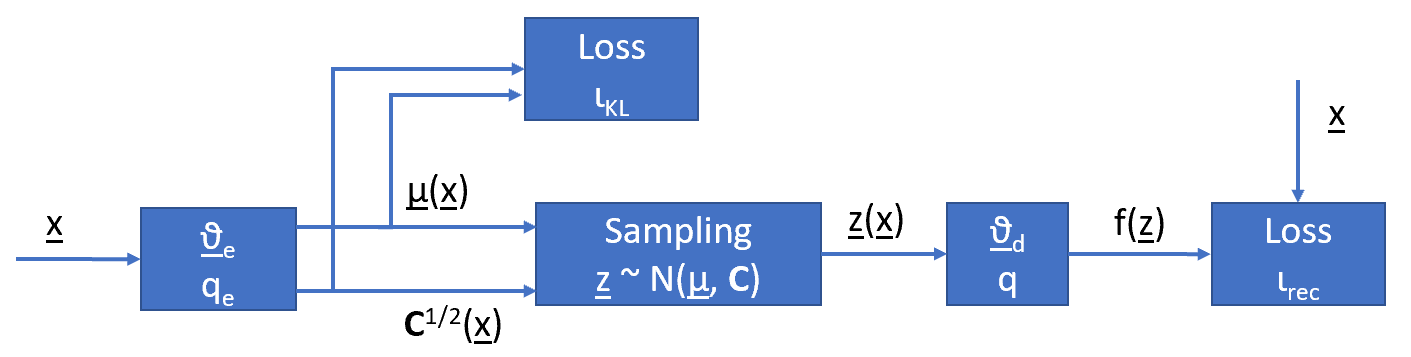
\includegraphics[width=0.75\linewidth]{Graphiken/VAE_wo_reparametrization}
	\caption{Sampling of $\underline{z}$ without reparametrization trick}
	\label{fig:Sampling_wo_reparametrization}
\end{figure}
This is fixed by using the reparametrization trick. Through this, it expresses the random variable $\underline{z}$ as a deterministic variable $\underline{z} = g(\underline{\epsilon}, \underline{x})$ where $\underline{\epsilon}$ is an auxiliary variable with independent marginal pdf $p(\underline{\epsilon})$. With an easy mapping of $\underline{z}$ (see equation \ref{eq:z_Mapping_reparametrization}) and $\underline{\epsilon} \backsim N(\underline{0}, \mathbf{I})$ the latent variable $\underline{z}$ can be calculated.
\begin{align}
	\underline{z} = g(\underline{\epsilon}, \underline{x}) = \underline{\mu} + \underline{\sigma}\cdot\underline{\epsilon}\label{eq:z_Mapping_reparametrization}
\end{align}
As a result of this trick, the non-linear sampling process is outside the path of the backpropagation. Thus $\underline{z}$ is now continuous in $\underline{\mu}$ and $\underline{\sigma}$ which are continuous in $\underline{\theta}_e$. So backpropagation is possible. This is visualized in figure \ref{fig:Sampling_w_reparametrization}.
\begin{figure}[htb!]
	\centering
	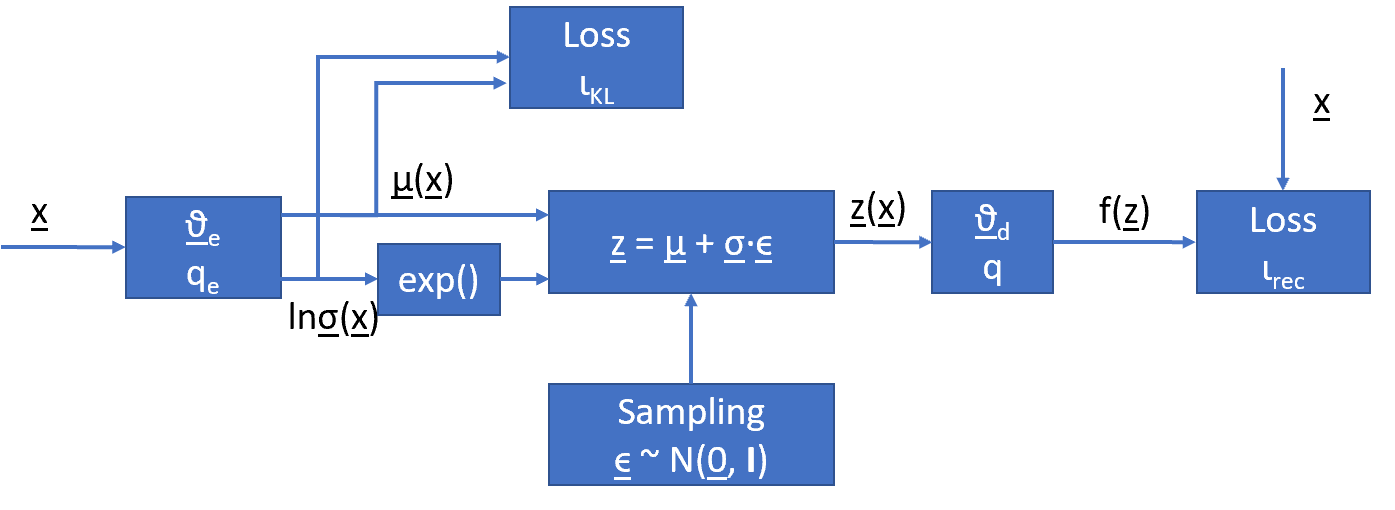
\includegraphics[width=0.75\linewidth]{Graphiken/VAE_w_reparametrization}
	\caption{Sampling of $\underline{z}$ with reparametrization trick}
	\label{fig:Sampling_w_reparametrization}
\end{figure}
Another trick is to use $\textrm{ln}(\underline{\sigma})$ instead of $\underline{\sigma}$, since $\underline{\sigma}$ is always non-negative while $\textrm{ln}(\underline{\sigma})$ can be positive and negative as $\underline{\mu}$, which is easier to output for the encoder. Also a diagonal $\mathbf{C} = \textrm{diag}(\underline{\sigma}\cdot\underline{\sigma})$ is assumed in figure \ref{fig:Sampling_w_reparametrization}. With these tricks and adoptions, an VAE can be easily trained via backpropagation (\cite{Kingma14VAE}, \cite{LectureNotes_DeepLearning}).
\section{Gumbel Variational Autoencoder}
The objective of clustering is representing the original data by a discrete structure of cluster assignments. Although categorical variables are often a natural choice for representing discrete structure in data, stochastic neural networks rarely use categorical latent variables due to the inability to backpropagate through those categorical samples. For this reason, \cite{Jang17GumbelVAE} introduce the so called Gumbel-Softmax distribution, which can on the one hand easily approximate categorical samples, on the other hand the gradients of it can be easily computed via the reparameterization trick. This will be used in this work to force an Variational Autoencoder having an approximately discrete latent space. A $k$-dimensional sample $\underline{y}$, drawn from the Gumbel-Softmax distribution can be generated with equation \ref{eq:GumbelSoftmax_Sample} with class probabilities $\pi$. $g_1...g_k$ are i.i.d samples drawn from Gumbel(0,1), which can be sampled as given in equation \ref{eq:Gumbel_Sample}.
\begin{align}
	y_i = \dfrac{\exp((\log(\pi_i)+g_i)/\tau}{\sum_{j=1}^{k}\exp((\log(\pi_i)+g_i)/\tau}\label{eq:GumbelSoftmax_Sample}
\end{align}
\begin{align}
	g = -\log(-\log(u)), u \backsim \textrm{Uniform(0,1)}\label{eq:Gumbel_Sample}
\end{align}
An adaptable parameter is the softmax temperature $\tau$. When $\tau$ approaches $0$, samples from Gumbel-Softmax become one-hot and the Gumbel-Softmax distribution becomes the categorical distribution. The distribution for different values of $\tau$ is shown in figure \ref{fig:Gumbel-Softmax_Distr}.
\begin{figure}[htb!]
	\centering
	\includegraphics[width=0.75\linewidth]{Graphiken/gumbel_temp_fig}
	\caption{Gumbel-Softmax distribution for different temperatures $\tau$ \cite{Jang17GumbelVAE}}
	\label{fig:Gumbel-Softmax_Distr}
\end{figure}
When implementing this modifications to the standard VAE architecture, the calculation of the loss and the generation of the latent representation $\underline{z}$ change slightly. The KL-Loss is now calculated between the new posterior distribution $q_e(\underline{z}|\underline{x};\underline{\theta}_e)$, which is a Softmax of the obtained logits and the new prior $q(\underline{z})$, where a uniform distributed data over the clusters is assumed. The logits are the output of the last encoder layer. The latent representation $\underline{z}$ is a sample drawn from the Gumbel-Softmax distribution (equation \ref{eq:GumbelSoftmax_Sample}) with \textit{logits} represents the output of the last encoder layer. This can be rewritten as equation \ref{eq:VAE_GumbelSoftmaxSample}.
\begin{align}
	z_i = \dfrac{\exp((logit+g_i)/\tau}{\sum_{j=1}^{k}\exp((logit+g_i)/\tau}\label{eq:VAE_GumbelSoftmaxSample}
\end{align}
With this setup, a VAE shall be forced to learn discrete latent representations of the data. The hyperparameter $\tau$ adjusts the \textit{discreteness} of the latent representation.
\section{IDEC}
As mentioned in previous chapters, the training of an autoencoder is not the best and natural choice for clustering, since the training is just performed based on the reconstruction loss. Therefore, many works add additional loss terms regarding the clustering perspective. One example, which is adding a clustering specific loss and performing clustering in parallel while training is the Improved Deep Emebedded Clustering (short IDEC) \cite{Guo17IDEC}. They propose a deep clustering algorithm that can jointly perform clustering and learn representations with local structure preservation. Therefore, the first step is pretraining a classical autoencoder, as described in section \ref{sec:AE}. After pre-training, the additional loss for deep embedding clustering is introduced, as proposed by \cite{Xie16DEC}. The fine-tuning of the encoder is done by optimizing the (clustering) objective in formula \ref{eq:Objective_DEC}.
\begin{align}
	L_c = \textrm{KL}(P||Q) = \sum_i\sum_j p_{ij}\log\dfrac{p_{ij}}{q_{ij}}\label{eq:Objective_DEC}
\end{align}
With $q_{ij}$ is the similarity between the latent representation $\underline{z}_i$ and the respective cluster center $\underline{\mu}_j$. As similarity measure the Student's $t$-distribution is used \cite{t-SNE} (formula \ref{eq:Student_t_similarity}).
\begin{align}
	q_{ij}=\dfrac{(1+||\underline{z}_i-\underline{\mu}_j||^2)^{-1}}{\sum_j(1+||\underline{z}_i-\underline{\mu}_j||^2)^{-1}}\label{eq:Student_t_similarity}
\end{align}
For assigning a latent representation $\underline{z}_i$ to a cluster, an arg max operation is executed. So the cluster with highest similarity is chosen. The assignment $s_i$ of sample $i$ is given in equation \ref{eq:IDEC_Assignment}.
\begin{align}
	s_i = \textrm{arg}\ \underset{j}\max\ q_{ij}\label{eq:IDEC_Assignment}
\end{align}

The target distribution $p_{ij}$ is defined in formula \ref{eq:IDEC_targetdistribution}.
\begin{align}
	p_{ij}=\dfrac{q_{ij}^{2}/\sum_i q_{ij}}{\sum_j q_{ij}^{2}/\sum_i q_{ij}}\label{eq:IDEC_targetdistribution}
\end{align}
This training procedure is a form of self-training, since the target distribution $P$ is defined by $Q$. With backpropagation, the latent representations $\underline{z}$ will be updated by updating the encoder parameters $\underline{\theta}_e$ as well as the cluster centers $\underline{\mu}_j$. IDEC additionally keeps the reconstruction loss $L_r$, to preserve the local structure. The overall Loss of IDEC is summarized by equation \ref{eq:IDEC_Loss}, with $\gamma > 0 $ is the hyperparameter that controls the degree of distorting embedding space.
\begin{align}
	L_{\textrm{IDEC}} = L_{r} + \gamma L_c\label{eq:IDEC_Loss}
\end{align}
When $\gamma = 1$ and $L_r = 0 $, the objective reduces to the objective from Deep Embedding Clustering (DEC) \cite{Xie16DEC}. The choice of the initial cluster centers is important for the convergence time and behaviour of IDEC. The centers are initialized by running K-means on the latent representations $\underline{z}$ based on the pretrained autoencoder. The observed cluster centers are then the initialization for $\underline{\mu}_j$. Since the target distribution $P$ is defined by $Q$, the target distribution has to be fixed for updating and training for a defined number of training steps. Than the target distribution and cluster assignments will be updated. This repeats for a defined number of epochs.
\chapter{Experimental Setup}
In this chapter, the set-up for running the experiments is described. Therefore, the Datasets are introduced, the used metrics and visualization tools for evaluation will be explained. Additionally, the investigated hyperparameters are shortly listed and the variation scheme is described. The results of these experiments will be given in a separate chapter.
\section{Datasets}
For evaluating the different experiments, six different datasets are used, which represent different complex datasets, thus resulting in different complex clustering tasks. It is important to mention, that in this work the datasets are divided into training and test dataset. Many works related to unsupervised learning and clustering put all together and train the model on one dataset. This can be done, since the network has never information about the label, so a remembering of an image label can not occur. However, the argumentation is that the models are trained on training data and the clustering step is performed on new unseen data. This allows to judge the generalization capability of the representation learning model, so it can be said that the feature extraction works also on unseen test data. The datasets and their splitting will be introduced shortly in table \ref{tab:Datasets}. For more details refer to the linked papers.
\begin{table}[htb!]
    \centering
    \caption{Datasets for experiments}
    \label{tab:Datasets}
    \begin{tabular}{lcccc}
        \toprule
        Dataset & \# Training images & \# Test images & Image Size & \# classes\\
        \midrule
        MNIST \cite{MNIST-Data} & 55000 & 10000 & 28x28x1 & 10\\
        F-MNIST \cite{xiao17F-MNIST} & 50000 & 10000 & 28x28x1 & 10\\
        CIFAR-10 \cite{Krizhevsky09CIFAR} & 50000 & 10000 & 32x32x3 & 10\\
        CIFAR-100 \cite{Krizhevsky09CIFAR} & 50000 & 10000 & 32x32x3 & 20\\
        Imagenet-Dog \cite{imagenet_cvpr09} & 19472 & 750 & 64x64x3 & 15\\
        Imagenet-10 \cite{imagenet_cvpr09} & 13000 & 500 & 64x64x3 & 10\\
        \bottomrule
    \end{tabular}
\end{table}
MNIST and Fashion MNIST are resized to 32x32x1 images, to keep the same comparative architecture for all datasets. Imagenet-Dog are 15 Dog classes drawn from the original Imagenet dataset with 1000 classes. This dataset is used to prove the performance of the clustering algorithm on similar data, since every class contain dogs. The 15 used classes are given as number labels, so that the dataset could easily be reproduced: 153, 156, 161, 174, 197, 207, 215, 216, 218, 224, 227, 230, 236, 254, 260.\\
Imagenet-10 are 10 randomly drawn classes from the entire Imagenet dataset. The 10 used classes are given as number labels, so that the dataset could easily be reproduced: 145, 153, 289, 404, 405, 510, 805, 817, 867, 950.
\section{Metrics and Visualization}
This section first introduces the metrics, which are used for evaluation of the experiments. After that, the visualization tools are described shortly. To compare clustering results fairly, different metrics are used. In this work the supervised metric Clustering accuracy (ACC) and the two unsupervised metrics Normalized Mutual Information (NMI) and Adjusted Rand Index (ARI) are used. Unsupervised means in this case, that no label information is needed to calculate the metric. Thus, when further choosing the best results, unsupervised metrics are referred, since unsupervised learning is performed, where in theory no label information is available. Additionally the clustering accuracy is given, since this is a metric which is well known and can be easily understood (50\% Accuracy means that 50\% of the data is clustered correctly). The metrics are calculated based on the whole test set in this work. Although algorithms with minibatches are used, the calculation of the metrics is done after clustering all test samples into the defined number of clusters. Otherwise, the batch size would directly influence the results, i.e. when choosing a small batch size $B$ which is nearly equal to the number of clusters $K$, the results would be very good, since every cluster will describe just a few samples.\\
Table \ref{tab:ClusterClassesmapping} represents a general mapping of cluster labels to class labels. More details about this and the usage of this information for metric calculation will be given in the following.
	\begin{table}[htb!]
    		\centering
    		\caption{Cluster to Classes mapping}
    		\label{tab:ClusterClassesmapping}
    		\begin{tabular}{l|cccc|c}
        		Cluster $\backslash$ Class & $Y_1$ & $Y_2$ & $\cdots$ & $Y_s$ & $Sums$\\ \hline
        		$C_1$ & $n_{11}$ & $n_{12}$ & $\cdots$ & $n_{1s}$ & $a_1$\\
        		$C_2$ & $n_{21}$ & $n_{22}$ & $\cdots$ & $n_{2s}$ & $a_2$\\
        		$\vdots$ & $\vdots$ & $\vdots$ & $\vdots$ & $\vdots$ & $\vdots$\\
        		$C_r$ & $n_{r1}$ & $n_{r2}$ & $\cdots$ & $n_{rs}$ & $a_r$\\ \hline
        		$Sums$ & $b_1$ & $b_2$ & $\cdots$ & $b_s$ & \\
    		\end{tabular}
	\end{table}
\begin{description}
	\item[Clustering Accuracy (ACC)]\hfill \\
	The clustering accuracy, sometimes also named purity, is a simple and transparent evaluation measure. To compute the clustering accuracy, each cluster $C$ is assigned to the class $Y$ which is most frequent in this cluster. Then the accuracy of this assignment is counted by easily computing the number of correctly assigned samples relative to the overall number of samples $N$. This can be written as given in formula \ref{eq:ClusterAccuracy} \cite{Manning08InformationRetrieval}.
	\begin{align}
		\textrm{ACC}(C,Y) = \dfrac{1}{N}\sum_{i=1}^s\underset{j}\max|C_i\cap Y_j|\label{eq:ClusterAccuracy}
	\end{align}
	\item[Normalized Mutual Information (NMI)]\hfill \\
	The mutual information $\textrm{I}(Y;C)$ of two random variables, here between the cluster assignments $C$ and the true class labels $Y$, quantifies the amount of information which can be obtained about one random variable by observing the other random variable. For clustering this is a measure how good the clustering reflects the true class labels. NMI is the normalized mutual information with the range between $0$ (bad clustering result) and $1$ (perfect clustering). The NMI is defined as in formula \ref{eq:NMI_general} with the mutual information $\textrm{I}(Y;C)$ and the entropies $\textrm{H}(Y)$ and $\textrm{H}(C)$ of the class labels or cluster labels respectively.
	\begin{align}
		\textrm{NMI}(Y,C) = \dfrac{2\textrm{I}(Y;C)}{\textrm{H}(Y)+\textrm{H}(C)}\label{eq:NMI_general}
	\end{align}
	Referring to table \ref{tab:ClusterClassesmapping}, the entropies for the cluster labels and class labels can be calculated with formula \ref{eq:Entropy_Cluster} and \ref{eq:Entropy_Class}.
	\begin{align}
		\textrm{H}(C) = -\sum_{i=1}^r\dfrac{a_i}{N}\log\dfrac{a_i}{N}\label{eq:Entropy_Cluster}\\
		\textrm{H}(Y) = -\sum_{j=1}^s\dfrac{b_j}{N}\log\dfrac{b_j}{N}\label{eq:Entropy_Class}
	\end{align}
	The mutual information $\textrm{I}(Y;C)$ can be calculated by equation \ref{eq:MutualInformation}.
	\begin{align}
		\textrm{I}(Y;C) = \sum_{i=1}^r\sum_{j=1}^s\dfrac{n_{ij}}{N}\log\dfrac{n_{ij}/N}{a_ib_j/N^2}\label{eq:MutualInformation}
	\end{align}
	Inserting equation \ref{eq:Entropy_Cluster}, \ref{eq:Entropy_Class} and \ref{eq:MutualInformation} in formula \ref{eq:NMI_general} yields the final NMI value \cite{Vinh10NMI}.
	\item[Adjusted Rand Index (ARI)]\hfill \\
	The ARI can be seen as corrected-for-chance version of the Rand Index \cite{Rand71RandIndex}. The adjusted Rand index is in range $-1$ to $1$. It takes the value $0$ when the index equals its expected value, $-1$ when the two distributions are totally different and $1$ when they are equal distributed. In general the ARI is given by formula \ref{eq:AdjustedRandIndex_general}.
	\begin{align}
		\textrm{ARI} = \dfrac{Index - ExpectedIndex}{MaxIndex - ExpectedIndex}\label{eq:AdjustedRandIndex_general}
	\end{align}
	When using ARI as unsupervised metric with no prior information, the classes are assumed to be uniform distribution, which is also the case in our datasets. The contingency table (table \ref{tab:ClusterClassesmapping}) gives the mapping from clusters to class labels. With this table now the specific ARI can be calculated, as given in formula \ref{eq:AdjustedRandIndex_specific} \cite{Yeung01ARI}.
	\begin{align}
		\textrm{ARI} = \dfrac{\sum_{ij}\binom{n_{ij}}{2}-[\sum_i\binom{a_i}{2}\sum_j\binom{b_j}{2}]/\binom{N}{2}}{\dfrac{1}{2}[\sum_i\binom{a_i}{2}+\sum_j\binom{b_j}{2}]-[\sum_i\binom{a_i}{2}\sum_j\binom{b_j}{2}]/\binom{N}{2}}\label{eq:AdjustedRandIndex_specific}
	\end{align}
\end{description} 
\section{Analysed Hyperparameters}
In this chapter the analysed hyperparameters and their modifications are described. As already mentioned previously, the hyperparameters can be split into two groups. The model-related ones and training specific ones.\\
In general, there exist a huge number of hyperparameters. Since all hyperparameters can possibly have an influence on another one, not all relevant combinations can be tested. Therefore the hyperparameters are (in the most cases) tested by their own and the value which yields the best results will be used for further experiments. First, the feature extraction models are adapted and optimized. Based on the optimized feature extraction models, the clustering models will be investigated.
\subsection{Model-related Hyperparameters}\label{subsec:Model-related Hyperparameters}
First, the model-related hyperparameters are investigated to find a good set-up to further improve the models by adapting the training-related hyperparameters. In the case of convolutional layers, the architecture-related hyperparameters are e.g. the kernel size, the filter size or the number of hidden layers. Due to time restrictions in this work, these are not further investigated. As base architecture the model drawn in \ref{fig:AE_ModelArchitecture} is used with 4 convolutional and one fully-connected layer and mirrored structure for encoder and decoder. The filter sizes are $16-32-64-128$ for the encoder and vice-versa for the decoder. Kernel size is set to $4$ and stride is $1$. Max pooling with $2x2$ pooling size for dimensionality reduction is used. The decoder uses deconvolution layers with kernel size $4$ and stride $2$.\\
In the following, it is described which hyperparameters will be investigated per introduced Model.
\begin{description}
	\item[Autoencoder]\hfill \\
	For the autoencoder, the influence of the latent size is investigated. Therefore the defined metrics over all datasets for different values of $n\_latent$ are evaluated: $[5, 10, 20, 32, 64, 128, 256]$.
	\item[Variational Autoencoder]\hfill \\
	For the variational autoencoder, the influence of the latent size is investigated. Therefore the defined metrics over all datasets for different values of $n\_latent$ are evaluated: $[5, 10, 20, 32, 64, 128, 256]$.
	\item[Discriminative Autoencoder]\hfill \\
	Base architecture is the autoencoder with the chosen best suitable $n\_latent$. Hyperparameters of the discriminative autoencoder are the weighting of the reconstruction loss $\lambda_r$ and the measure for the uncertainty of the anchor pairs $\alpha$. They both influence directly the loss and so the optimization task. Thus they are tested jointly in a grid search. $\alpha$ is set to the values $[0, 0.5, 1]$ and $\lambda_r$ to $[10, 1, 0.1, 0.01, 0.001]$. This results in $15$ tests per dataset. In \cite{DiscriminativeClustering}, they propose a value of $0.001$ for $\lambda_r$ for MNIST, but no value for $\alpha$ is given.
	\item[Gumbel Variational Autoencoder]\hfill \\
	For the Gumbel VAE, the temperature $\tau$ is a hyperparameter. Since $\tau$ directly influences the latent space, this hyperparameter is investigated jointly with the size of the latent space $n\_latent$ by a grid search. $\tau$ is therefore set to $[10, 5, 2, 1]$ and $n\_latent$ to $[5, 10, 64]$. This gives $15$ runs per dataset.
	\item[K-Means]\hfill \\
	For the implemented clustering algorithm K-Means, the following hyperparameters are investigated. The number of clusters $K$ directly influence the clustering performance. Therefore $K$ is set to the values $[5, 10, 15, 20, 50]$, to have tests with less clusters than real classes and with much more clusters than true classes. In addition, the effect of the batch size to the minibatch K-Means algorithm is analysed. Therefore the clustering batch size $B_{cluster}$ is set to the values $[64, 500, 1024, 2048]$.
\end{description}
\subsection{Training-related Hyperparameters}\label{subsec:Training-related Hyperparameters}
The training of a deep neural network can be optimized and adapted on a wide range of hyperparameters. Typical examples which directly influence the training procedure are the minibatch size, the choice of the optimizer with its parameters (i.e. Momentum), the learning rate choice or a learning rate schedule, the parameter initialization, number of epochs or methods like batch normalization or input scaling. In this work, the focus is on optimizing the training procedure of the latent models. As mentioned, a lot of possible hyperparameters can be adapted and optimized. Due to time restrictions, not all of them can be optimized. In the following, the investigated hyperparameters will be described and in which form the variation will take place.
\begin{description}
	\item[Batch Size]\hfill \\
	Based on the samples inside a batch, the (noisy) gradient is calculated for further optimization of the network. Therefore it is clear, that the batch size directly influences the learning procedure of a deep neural network. Following \cite{Goodfellow-et-al-2016}, the minibatch sizes are driven by  different factors, i.e. that larger batches provides a more accurate estimate of the gradient, but with less than linear returns. It is also mentioned there, that small batches can offer a regularization effect, which often lead to a better generalization error with decreasing batch size. The reason for this can be the introduced noise through small batch sizes. Also it should be mentioned, that the batch size directly influence the memory consumption, so in general it is desired to use small batch sizes for faster computation and less memory consumption. In this work batch sizes in the range from 64 to 1024 are compared, more precisely the following values are investigated: $[64, 128, 256, 512, 1024]$.\\ As the batch size directly influence the gradient calculation, and thus the optimization step, these values are jointly optimized with different learning rates, since a more noisy gradient perhaps needs a smaller step size for convergence \cite{Goodfellow-et-al-2016}.
	\item[Constant Learning Rate]\hfill \\
	As mentioned before and introduced in the beginning of the work, the optimization step depends on the learning rate $\gamma$, often also called step size. Different ways to vary the learning rate are used. Here the constant learning rates are varied. In a separate part different learning rate schedules are proposed. The fixed learning rates are analysed jointly with the above defined batch sizes via a grid search. The values for the learning rate $\gamma$ are $[0.001, 0.01, 0.1]$.
	\item[Learning Rate Schedule]\hfill \\
	What can be a remaining challenge when having a constant learning rate, is a possible slow convergence with a small learning rate or an oscillation around a local minima with too large learning rates. Therefore a compromise between a fast convergence at the beginning (high learning rate) and an accurate update around the local minima (low learning rate) is desired. To combine both points, learning rate schedules are used, where the learning rate $\gamma$ decays over the number of epochs following a specific schedule. Different schedules are used and their effect on clustering is investigated. The different schedules will be introduced in the following.
	\begin{description}
		\item[Step decay]\hfill \\Step decay steps down the learning rate, as it name says. After a defined time interval $t_0$, the learning rate steps down to $c\cdot\gamma_0$ with the decay factor $c$ and the initial learning rate $\gamma_0$. Then the time interval starts again and the next decay, leading to the learning rate $c^2\cdot\gamma_o$ takes place at $2t_0$ \cite{LectureNotes_DeepLearning}. The values for the time interval $t_0$, initial learning rate $\gamma_0$ and the decay factor $c$ will be defined based on the results obtained from previous defined experiments (e.g. from constant learning rate experiments).
		\item[Exponential decay]\hfill \\The exponential decay has an exponential learning rate curve starting from $t_0$. Before, the learning rate is constant. The learning rate with exponential can be calculated as stated in formula \ref{eq:ExponentialDecay} \cite{LectureNotes_DeepLearning}.
		\begin{align}
			\gamma(t) = \begin{cases} \gamma_0 & t \leq t_0\\\gamma_0\textrm{e}^{-c(t-t_0)} & t > t_0\\ \end{cases}\label{eq:ExponentialDecay}
		\end{align}
		The values for the time interval $t_0$, initial learning rate $\gamma_0$ and the decay factor $c$ will be defined based on the results obtained from previous defined experiments (e.g. from constant learning rate experiments).
		\item[Triangular Learning Rate]\hfill \\This learning rate is a cyclic learning rate, which periodically perform the same learning rate schedule. As given in \cite{Smith15CyclicLearningRate}, different numerical functional forms for the cyclic adoption are possible (i.e. triangular window, welch window, and a hann window) and they all produce equivalent results. That's why the mathematical easiest function will be used, the triangular learning rate. The learning rate inside the stepsize $t_0$ can be described by equation \ref{eq:Lr_Triangular} with the sign and $\gamma_0$ depending on the step (in this work, for odd steps the sign is positive and $\gamma_0 = base\_lr$, so learning rate starts at $base\_lr$).
		\begin{align}
			\gamma(t) = \gamma_0\pm\dfrac{max\_lr-base\_lr}{t_0}t\label{eq:Lr_Triangular}
		\end{align}		
		The learning rate schedule is visualized in figure \ref{fig:Triangular Learning rate}. The blue line represent the learning rate values changing between the bounds. The parameter for $t_0$ is the number of iterations in half a cycle. The bounds $max\_lr$ and $base\_lr$ are the defined maximum or minimum learning rates. The values for the maximum and minimum learning rate will be defined based on the results obtained from previous defined experiments (e.g. from constant learning rate experiments).
		\begin{figure}[htb!]
			\centering
			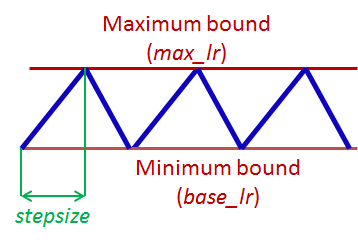
\includegraphics[width=0.3\linewidth]{Graphiken/triangularWindow}
			\caption{Triangular learning rate schedule \cite{Smith15CyclicLearningRate}}
			\label{fig:Triangular Learning rate}
		\end{figure}
		\item[Linear Warmup]\hfill \\Learning rate warmup is a common heuristic used by many works for training deep neural networks. Warmup is motivated to use large learning rates without causing training instability \cite{gotmare2018Warmup}. As it just influence the warmup, it can be used in combination with any other schedule. In this work a linear warmup starting from $0$ to $\gamma_0$ over a defined interval $t_0$ will be used. The learning rate in the time interval $[0, t_0]$ is defined in formula \ref{eq:Lr_Warmup}.
		\begin{align}
			\gamma(t) = \dfrac{\gamma_0}{t_0}t\label{eq:Lr_Warmup}
		\end{align}
		The parameters $\gamma_0$ and $t_0$ will be defined based on the results obtained from previous defined experiments (e.g. from constant learning rate experiments).
	\end{description}
\end{description}
\chapter{Experiments and Results}
In this chapter, the specific experiments and their results will be described. Since all possible variations of the hyperparameters for all models on all datasets would result in a tremendous amount of runs, the optimization is done on specific models, namely based on the standard autoencoder and variational autoencoder which are introduced above, since they are the base for the adapted models. Nevertheless, obtained optimal parameters will also be checked on the other models.\\
The latent models are trained for 50 epochs on the training dataset using the Adam optimizer with the default values $\beta_1=0.9$, $\beta_2=0.999$ and $\epsilon = 1x10^{-8}$ \cite{Kingma14AdamOptimizer}. The clustering algorithm is trained on the test dataset for 20 epochs, if not mentioned explicitly. The obtained results base on unseen test dataset. As clustering algorithm K-means will be used. The number of clusters is set to the original class number, if not explicitly mentioned.\\
\section{Model-related Hyperparameters}
As introduced in subsection \ref{subsec:Model-related Hyperparameters}, the different defined model-related hyperparameters will be analysed and the optimum parametetrization for the different models will be defined. 
\paragraph{Autoencoder \& Variational Autoencoder}\hfill \\
As given and introduced in the previous chapter, for the autoencoder and the variational autoencoder, the effect of the latent size is checked with respect to the clustering performance. Therefore the other hyperparameters are fixed and the value of $n_{latent}$ is set to $[5, 10, 20, 32, 64, 128, 256]$. The other hyperparameters are set to the following values: $batchsize_{training} = 256$, $batchsize_{clustering} = 500$, $\gamma_0 = 0.001$. Figure \ref{fig:ClusterPerformance_latentSpace} shows exemplary the NMI values for the MNIST (\ref{fig:ClusterNMI_MNIST_n_latent}) and CIFAR-10 (\ref{fig:ClusterNMI_CIFAR-10_n_latent}) dataset.
	\begin{figure}[htb!]
		\centering
		\subfloat[Cluster Accuracy\label{fig:ClusterNMI_MNIST_n_latent}]{%	
		\resizebox{0.45\linewidth}{!}{% This file was created by matplotlib2tikz v0.7.4.
\begin{tikzpicture}

\begin{axis}[
legend cell align={left},
legend style={draw=white!80.0!black},
tick align=outside,
tick pos=left,
title={Clustering performance of AE VAE at MNIST},
x grid style={white!69.01960784313725!black},
xlabel={n\_latent},
xmin=-7.55, xmax=268.55,
xtick style={color=black},
y grid style={white!69.01960784313725!black},
ylabel={NMI},
ymin=0, ymax=1,
ytick style={color=black}
]
\addplot [semithick, red]
table {%
5 0.789449155330658
10 0.744279801845551
20 0.654446125030518
32 0.559625446796417
64 0.524512648582458
128 0.529116988182068
256 0.519109606742859
};
\addlegendentry{AE}
\addplot [semithick, blue]
table {%
5 0.728410959243774
10 0.662225484848022
20 0.532534837722778
32 0.515085995197296
64 0.39774963259697
128 0.132218912243843
256 0.0114405900239944
};
\addlegendentry{VAE}
\end{axis}

\end{tikzpicture}}}
		\qquad
		\subfloat[Normalized Mutual Information\label{fig:ClusterNMI_CIFAR-10_n_latent}]{%			
		\resizebox{0.45\linewidth}{!}{% This file was created by matplotlib2tikz v0.7.4.
\begin{tikzpicture}

\begin{axis}[
legend cell align={left},
legend style={draw=white!80.0!black},
tick align=outside,
tick pos=left,
title={Clustering performance of AE VAE at CIFAR-10},
x grid style={white!69.01960784313725!black},
xlabel={n\_latent},
xmin=-7.55, xmax=268.55,
xtick style={color=black},
y grid style={white!69.01960784313725!black},
ylabel={NMI},
ymin=0, ymax=1,
ytick style={color=black}
]
\addplot [semithick, red]
table {%
5 0.0899999439716339
10 0.104692973196507
20 0.109597973525524
32 0.0841954052448273
64 0.0873732045292854
128 0.0757577270269394
256 0.0780473873019218
};
\addlegendentry{AE}
\addplot [semithick, blue]
table {%
5 0.0941048413515091
10 0.119100347161293
20 0.100977852940559
32 0.0942699462175369
64 0.0708507969975471
128 0.0451396480202675
256 0.0331674069166183
};
\addlegendentry{VAE}
\end{axis}

\end{tikzpicture}}}
		\caption{Clustering Performance (NMI) for AE/VAE + K-means on different sizes of latent space for MNIST and CIFAR-10}
		\label{fig:ClusterPerformance_latentSpace}
	\end{figure}
For MNIST, it can be obtained that a smaller latent space increases the final clustering performance in this set-up. But it has to be taken care, that this does not necessary holds in general for all clustering algorithms. For a higher dimensional latent space (i.e. $n_{latent} = 256$), a clustering algorithm based on distances as K-means could have problems to determine meaningful distances in this high-dimensional space (also denoted as "course of dimensionality"). Also it can be seen, that a VAE is much more sensitive to higher dimensional latent spaces, since there the NMI approaches $0$, while the AE stays almost stable from $n_{latent} = 64$ onwards. Based on the executed experiments it seems, that the smaller the bottleneck is, the more it is enforcing the feature extraction model to generate meaningful latent representations $\underline{z}$. From a clustering point of view, this is an important and relevant point. In addition, the difference of the datasets can be seen and that one dataset is not enough to produce a meaningful statement. In example, at CIFAR-10, the gain of clustering performance for lower sizes of latent space is much lower than for MNIST.\\
On the other side it is obvious, that smaller latent spaces resulting in a harder job for the decoder to decode this low dimensional representation to the original image. This is proved by figure \ref{fig:TestLoss_AE_latentSpace}, which shows the test loss of the autoencoder for different $n_{latent}$ at the MNIST dataset (figure \ref{fig:TestLoss_AE_latentSpace_MNIST}) and CIFAR-10 dataset (figure \ref{fig:TestLoss_AE_latentSpace_CIFAR-10}).
	\begin{figure}[htb!]
		\centering
		\subfloat[MNIST\label{fig:TestLoss_AE_latentSpace_MNIST}]{%
		\resizebox{0.45\linewidth}{!}{% This file was created by matplotlib2tikz v0.7.4.
\begin{tikzpicture}

\begin{axis}[
legend cell align={left},
legend style={draw=white!80.0!black},
tick align=outside,
tick pos=left,
title={test loss of AE at MNIST},
x grid style={white!69.01960784313725!black},
xlabel={n\_latent},
xmin=-7.55, xmax=268.55,
xtick style={color=black},
y grid style={white!69.01960784313725!black},
ylabel={test\_loss},
ymin=0.000538408855209127, ymax=0.0156523040670436,
ytick style={color=black}
]
\addplot [semithick, red]
table {%
5 0.014965308830142
10 0.00681421812623739
20 0.00344323040917516
32 0.00236964877694845
64 0.00143344863317907
128 0.00133219780400395
256 0.00122540409211069
};
\addlegendentry{AE}
\end{axis}

\end{tikzpicture}}}
		\qquad
		\subfloat[CIFAR-10\label{fig:TestLoss_AE_latentSpace_CIFAR-10}]{%			
		\resizebox{0.45\linewidth}{!}{% This file was created by matplotlib2tikz v0.7.4.
\begin{tikzpicture}

\begin{axis}[
legend cell align={left},
legend style={draw=white!80.0!black},
tick align=outside,
tick pos=left,
title={test loss of AE at CIFAR-10},
x grid style={white!69.01960784313725!black},
xlabel={n\_latent},
xmin=-7.55, xmax=268.55,
xtick style={color=black},
y grid style={white!69.01960784313725!black},
ylabel={test loss},
ymin=0.00399183803237975, ymax=0.0276239119004458,
ytick style={color=black}
]
\addplot [semithick, red]
table {%
5 0.0265497267246246
10 0.0201517660170794
20 0.0148076489567757
32 0.0118082966655493
64 0.00817384757101536
128 0.00576603598892689
256 0.00506602320820093
};
\addlegendentry{AE}
\end{axis}

\end{tikzpicture}}}
		\caption{Test Loss of the AE on different sizes of latent space at MNIST and CIFAR-10}
		\label{fig:TestLoss_AE_latentSpace}
	\end{figure}
This effect can also be seen at the reconstructed images. Therefore figure \ref{fig:Reconstructions_nLatent} shows exemplary one original image (\ref{fig:CIFAR-10_OriginalImage}) from CIFAR-10 and the reconstructed images after 50 training epochs for $n_{latent}=5$ (\ref{fig:CIFAR-10_nLatent_5}), $n_{latent}=32$ (\ref{fig:CIFAR-10_nLatent_32}) and $n_{latent}=256$ (\ref{fig:CIFAR-10_nLatent_256}). The image is drawn from the CIFAR-10 dataset, to show this effect on a more difficult image (i.e. colored) than on an \textit{easy} sample like from MNIST, where the difference can't be seen directly at the reconstructed images.
\begin{figure}[htb!]
	\centering
	\subfloat[Original Image\label{fig:CIFAR-10_OriginalImage}]{%			
		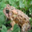
\includegraphics[width=0.1\linewidth]{Graphiken/CIFAR-10_OriginalImage}}
	\qquad
	\subfloat[$n_{latent}=5$\label{fig:CIFAR-10_nLatent_5}]{%			
		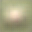
\includegraphics[width=0.1\linewidth]{Graphiken/CIFAR-10_Recon_nlatent_5}}
	\qquad
	\subfloat[$n_{latent}=32$\label{fig:CIFAR-10_nLatent_32}]{%			
		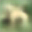
\includegraphics[width=0.1\linewidth]{Graphiken/CIFAR-10_Recon_nlatent_32}}
	\qquad
	\subfloat[$n_{latent}=256$\label{fig:CIFAR-10_nLatent_256}]{%			
		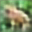
\includegraphics[width=0.1\linewidth]{Graphiken/CIFAR-10_Recon_nlatent_256}}
	\qquad
	\caption{Original and reconstructed images for different $n_{latent}$}
	\label{fig:Reconstructions_nLatent}
\end{figure}
These images show directly the impact of the different latent spaces for the reconstructions. While the smallest latent space ($n_{latent}=5$) can just provide some deviations of colour without any visible edges or shapes, $n_{latent}=32$ provides already the shapes of the frog and a distinction between the frog and the background. With a latent space size of $256$, it can be already detected that a frog is at the picture and more details like the eye can be reconstructed.
As it can be seen in figure \ref{fig:TestLoss_AE_latentSpace}, a latent space with $n_{latent}=10$ reduces for MNIST the test loss already by circa a half in comparison to a size of $5$. To show the effect of the latent space size on the different datasets, table \ref{tab:ClusterACC_n_latent} summarizes the clustering accuracies obtained on the different datasets with different values of $n_{latent}$ indicating the best result per dataset in \textbf{bold}.
	\begin{table}[htb!]
    		\centering
    		\caption{Clustering Accuracy in \% of autoencoder + K-means on different datasets with different latent space sizes}
    		\label{tab:ClusterACC_n_latent}
    		\begin{tabular}{l|ccccccc}
        		Dataset $\backslash$ $n_{latent}$ & $5$ & $10$ & $20$ & $32$ & $64$ & $128$ & $256$\\ \hline
        		MNIST & $\mathbf{87.2}$ & $79.5$ & $73.6$ & $65.8$ & $64.0$ & $64.7$ & $64.2$\\
        		F-MNIST & $\mathbf{63.3}$ & $62.0$ & $58.4$ & $57.7$ & $56.9$ & $61.9$ & $61.8$\\
        		CIFAR-10 & $23.4$ & $24.6$ & $\mathbf{24.9}$ & $23.1$ & $23.3$ & $22.1$ & $22.3$\\
        		CIFAR-100 & $14.4$ & $15.7$ & $15.8$ & $\mathbf{16.2}$ & $15.8$ & $17.7$ & $15.0$\\
        		Imagenet-10 & $24.1$ & $23.9$ & $\mathbf{25.8}$ & $25.0$ & $23.1$ & $25.4$ & $23.6$\\
        		Imagenet-Dog & $19.0$ & $21.1$ & $20.5$ & $20.9$ & $20.9$ & $20.9$ & $\mathbf{22.1}$\\
    		\end{tabular}
	\end{table}
Further in this work, a latent size of $10$ is used, since good clustering results are achieved with this setup and the reconstruction loss can be reduced clearly in comparison to a even smaller latent space, i.e. $5$. Also for more complex datasets (e.g. Imagenet-Dog) a to small latent space seems to reduce the clustering performance.
	\paragraph{Discriminative Autoencoder}\hfill \\
	Based on the obtained latent size $n_{latent} = 10$, the hyperparmeters of the discriminative autoencoder are evaluated. Therefore the parameters $\alpha$ and $\lambda_r$ are varied. Out of the training batch size, which is set to $1000$, the other hyperparameters stays as described for the AE and VAE. The high batch size is necessary, so that the assumption about uniform distributed samples over the different classes inside a batch holds.
	\\Figure \ref{fig:ClusterPerformance_b_AE_Hyperparameters} shows the resulting NMI values for the different settings of the hyperparameters for MNIST (\ref{fig:MNIST_NMI_b_AE_alpha_lambda}) and Imagenet-10 (\ref{fig:IMAGENET10_NMI_b_AE_alpha_lambda}).
	\begin{figure}[htb!]
		\centering
		\subfloat[NMI MNIST\label{fig:MNIST_NMI_b_AE_alpha_lambda}]{%	
		{\includegraphics[width=0.45\linewidth]{Graphiken/MNIST_discriminative_AE_NMI_alpha_lambda_r}}}
		\qquad
		\subfloat[NMI Imagenet-10\label{fig:IMAGENET10_NMI_b_AE_alpha_lambda}]{%			
		{\includegraphics[width=0.45\linewidth]{Graphiken/IMAGENET-10_discriminative_AE_NMI_alpha_lambda_r}}}
		\caption{Clustering Performance (NMI) for discriminative AE + K-means on different $\alpha$ and $\lambda_r$ for MNIST and Imagenet-10}
		\label{fig:ClusterPerformance_b_AE_Hyperparameters}
	\end{figure}
	Following the behaviour of the NMI and the clustering objective, the hyperparameters $\lambda_r = 1$ and $\alpha=0.5$ are chosen, since these values give good clustering results for the different dataset. Referring to \cite{DiscriminativeClustering}, $\lambda_r = 0.001$ is proposed. But in this paper, the reconstruction loss is not normalized with the number of samples per minibatch, so for a batch size of $1000$ as used in this experiment, $\lambda_r$ equals the setup proposed by the paper. Nevertheless, with the current setup, a clustering accuracy of $92\%$ can't be achieved within 50 epochs, as claimed in the original paper.
	\paragraph{Gumbel Variational Autoencoder}\hfill \\
	The main hyperparameter for the Gumbel VAE is the temperature $\tau$ of the Gumbel Softmax distribution. Since the Gumbel distributions changes directly the Latent Space, also the latent space is slighty varied. These two hyperparameters are investigated jointly for $\tau = [10, 5, 2, 1]$ and $n_{latent} = [5, 10, 20]$. The corresponding results and effect on clustering performance can be seen in figure \ref{fig:ClusterPerformance_g_VAE_Hyperparameters} for the two datasets MNIST (\ref{fig:MNIST_NMI_g_VAE_tau_nlatent}) and Imagenet-10 (\ref{fig:IMAGENET10_NMI_g_VAE_tau_nlatent}). In figure \ref{fig:MNIST_NMI_g_VAE_tau_nlatent}, two observation points for $\tau=10$, $n_{latent}=5$ and $\tau=1$, $n_{latent}=64$ are missing. Due to time restrictions these experiments couldn't be repeated, but based on observations for these working points at other datasets, it can be accepted since at these combinations worse clustering performance is seen.
	 \begin{figure}[htb!]
		\centering
		\subfloat[NMI MNIST\label{fig:MNIST_NMI_g_VAE_tau_nlatent}]{%	
		{\includegraphics[width=0.45\linewidth]{Graphiken/MNIST_Gumbel_VAE_NMI_n_latent_temperature_gumbel}}}
		\qquad
		\subfloat[NMI Imagenet-10\label{fig:IMAGENET10_NMI_g_VAE_tau_nlatent}]{%			
		{\includegraphics[width=0.45\linewidth]{Graphiken/IMAGENET-10_Gumbel_VAE_NMI_n_latent_temperature_gumbel}}}
		\caption{Clustering Performance (NMI) for Gumbel VAE + K-means on different $\tau$ and $n_{latent}$ for MNIST and Imagenet-10}
		\label{fig:ClusterPerformance_g_VAE_Hyperparameters}
	\end{figure}
	The hyperparameter $n_{latent}$ stays fixed at value $10$ due to previous observation and comparability to the other architectures. But it can be seen that the size of $n_{latent}$ correlates with the temperature $\tau$. With given $n_{latent}=10$, the temperature is set to $\tau=10$ based on the results of figure \ref{fig:MNIST_NMI_g_VAE_tau_nlatent}. For $n_{latent}=10$, the effect of the temperature $\tau$ for the discreteness of the latent representation $\underline{z}$ is visualized in figure \ref{fig:Different_GumbelTemperatures} with the corresponding original image (\ref{fig:OriginalImage_g_VAE}) drawn from the Imagenet-10 dataset.
	\begin{figure}[htb!]
	\centering
	\subfloat[Original Image\label{fig:OriginalImage_g_VAE}]{%			
		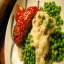
\includegraphics[width=0.15\linewidth]{Graphiken/Imagenet-10_OriginalImage_g_VAE}}
	\qquad
	\subfloat[$\tau=1$\label{fig:z_tau_1}]{%			
		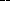
\includegraphics[width=0.2\linewidth]{Graphiken/Imagenet-10_latentspace_tau1_g_VAE}}
	\qquad
	\subfloat[$\tau=2$\label{fig:z_tau_2}]{%			
		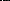
\includegraphics[width=0.2\linewidth]{Graphiken/Imagenet-10_latentspace_tau2_g_VAE}}
	\qquad
	\subfloat[$\tau=5$\label{fig:z_tau_5}]{%			
		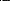
\includegraphics[width=0.2\linewidth]{Graphiken/Imagenet-10_latentspace_tau5_g_VAE}}
	\qquad
	\subfloat[$\tau=10$\label{fig:z_tau_10}]{%			
		
\includegraphics[width=0.2\linewidth]{Graphiken/Imagenet-10_latentspace_tau10_g_VAE}}
	\qquad
	\caption{Original iamge and latent space for different values of $\tau$}
	\label{fig:Different_GumbelTemperatures}
\end{figure}
The figures shows the latent representation for the different temperature values $1$ (\ref{fig:z_tau_1}), $2$ (\ref{fig:z_tau_2}), $5$ (\ref{fig:z_tau_5}) and $10$ (\ref{fig:z_tau_10}) after 50 epochs of training on Imagenet-10. The pixels represent the different neurons of the latent layer with a white pixel indicating an active neuron and black inactive. For $\tau = 10$ the activations are distributed over the different neurons, while for $\tau = 1$ a discrete latent representation $\underline{z}$ of the original input image is achieved. This effect can also be visualised using an UMAP transformation into 2-d space of the above shown latent representations. This is illustrated in figure \ref{fig:Different_GumbelTemperatures_UMAP}.
	\begin{figure}[htb!]
	\centering
	\subfloat[$\tau=1$\label{fig:UMAP_z_tau_1}]{%			
		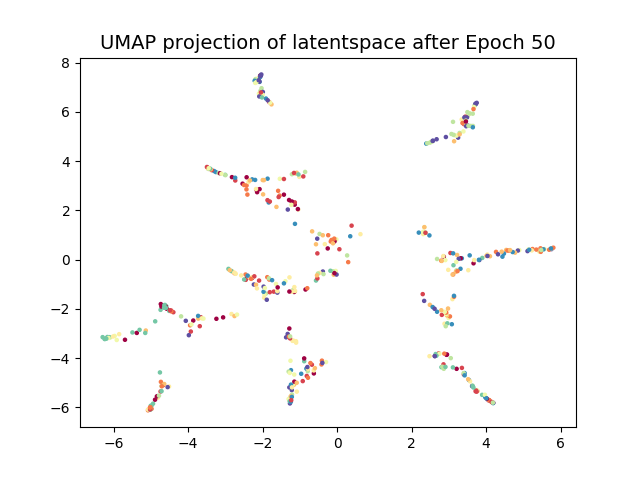
\includegraphics[width=0.4\linewidth]{Graphiken/Imagenet-10_latentspace_tau1_UMAP_g_VAE}}
	\qquad
	\subfloat[$\tau=2$\label{fig:UMAP_z_tau_2}]{%			
		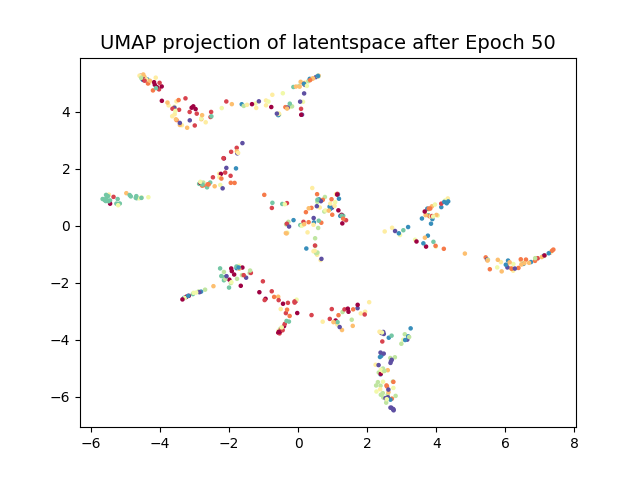
\includegraphics[width=0.4\linewidth]{Graphiken/Imagenet-10_latentspace_tau2_UMAP_g_VAE}}
	\qquad
	\subfloat[$\tau=5$\label{fig:UMAP_z_tau_5}]{%			
		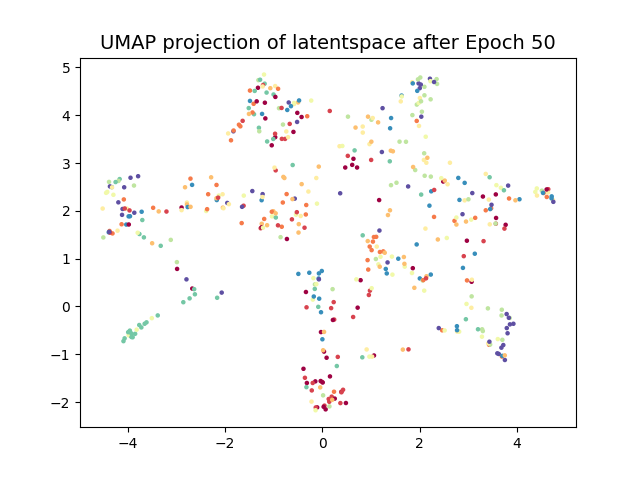
\includegraphics[width=0.4\linewidth]{Graphiken/Imagenet-10_latentspace_tau5_UMAP_g_VAE}}
	\qquad
	\subfloat[$\tau=10$\label{fig:UMAP_z_tau_10}]{%			
		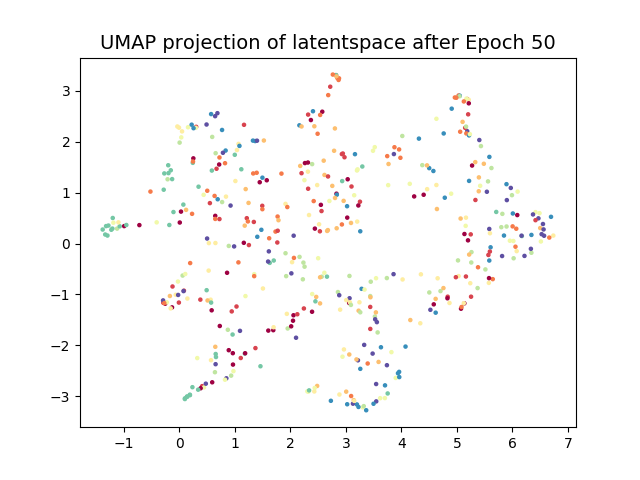
\includegraphics[width=0.4\linewidth]{Graphiken/Imagenet-10_latentspace_tau10_UMAP_g_VAE}}
	\qquad
	\caption{UMAP-transformed latent space for different values of $\tau$}
	\label{fig:Different_GumbelTemperatures_UMAP}
\end{figure}
It shows the intention why using discrete latent representations for clustering could be a good thing. The samples from figure \ref{fig:UMAP_z_tau_1} seems to represent already different clusters, while in figure \ref{fig:UMAP_z_tau_10} the samples are distributed continuously in the latent space. A possible useful adoption of the Gumbel VAE could be that additional information to the encoder is delivered to encode similar original images to the same discrete latent representation. Due to time restrictions in this work, no further adoptions and improvements on the architecture of the Gumbel VAE could be done.\\
Up to now, the model-related hyperparameters are optimized. In table \ref{tab:ClusterPerformance_Models_ModelrelatedParams} the performances of the different models are summarized with the above mentioned chosen hyperparameters. The best model per dataset and metric is marked in \textbf{bold}. This will be seen as base for further optimization of the clustering performance by adapting the training-related hyperparamters.
	\begin{table}[htb!]
    		\centering
    		\caption{Clustering Performance of models + K-means on different datasets with chosen hyperparameters}
    		\label{tab:ClusterPerformance_Models_ModelrelatedParams}
    		\begin{tabular}{l|ccccccccc}
    			\toprule
    			\multicolumn{1}{c}{Dataset} & \multicolumn{3}{c}{MNIST} & \multicolumn{3}{c}{F-MNIST} & \multicolumn{3}{c}{CIFAR-10}\\
        		\multicolumn{1}{c}{Metric} & ACC & NMI & ARI & ACC & NMI & ARI & ACC & NMI & ARI\\
        		\midrule
    			AE & $\mathbf{0.80}$ & $\mathbf{0.74}$ & $\mathbf{0.68}$ & $0.62$ & $\mathbf{0.62}$ & $\mathbf{0.45}$ & $0.25$ & $0.10$ & $0.06$\\
        		discriminative AE & $0.77$ & $0.71$ & $0.63$ & $\mathbf{0.64}$ & $0.61$ & $0.44$ & $0.24$ & $0.09$ & $0.05$\\
        		VAE & $\mathbf{0.80}$ & $0.66$ & $0.62$ & $0.57$ & $0.50$ & $0.38$ & $\mathbf{0.26}$ & $\mathbf{0.12}$ & $\mathbf{0.07}$\\
        		Gumbel VAE & $0.60$ & $0.50$ & $0.39$ & $0.47$ & $0.44$ & $0.28$ & $0.21$ & $0.08$ & $0.04$\\
        		\bottomrule
    		\end{tabular}    		
    		\begin{tabular}{l|ccccccccc}
    			\toprule
    			\multicolumn{1}{c}{Dataset} & \multicolumn{3}{c}{CIFAR-100} & \multicolumn{3}{c}{Imagenet-10} & \multicolumn{3}{c}{Imagenet-Dog}\\
        		\multicolumn{1}{c}{Metric} & ACC & NMI & ARI & ACC & NMI & ARI & ACC & NMI & ARI\\
        		\midrule
    			AE & $\mathbf{0.16}$ & $\mathbf{0.09}$ & $\mathbf{0.04}$ & $0.24$ & $0.11$ & $0.04$ & $0.21$ & $0.14$ & $0.04$\\
        		discriminative AE & $0.11$ & $0.05$ & $0.01$ & $0.26$ & $\mathbf{0.15}$ & $0.05$ & $0.17$ & $0.10$ & $0.02$\\
        		VAE & $\mathbf{0.16}$ & $\mathbf{0.09}$ & $0.03$ & $\mathbf{0.27}$ & $\mathbf{0.15}$ & $\mathbf{0.06}$ & $\mathbf{0.22}$ & $\mathbf{0.15}$ & $\mathbf{0.05}$\\
        		Gumbel VAE & $0.14$ & $0.08$ & $0.02$ & $0.25$ & $0.12$ & $0.04$ & $0.20$ & $0.14$ & $0.03$\\
        		\bottomrule
    		\end{tabular}
	\end{table}
	Shortly, it can be stated, that the classical autoencoder produces better results for MNIST and F-MNIST, while the VAE enables sligthly better clustering performance on colored images (CIFAR-10, CIFAR-100, Imagenet-10, Imagenet-Dog).
\section{Training-related Hyperparameters}
In this section, the above introduced training-related hyperparameters, mainly the learning rate, will be analysed and optimized with respect to the clustering objective of this work. A big impact of the learning rate is expected, since it clearly changes and hopefully improves the training procedure. The model-related hyperparameters are fixed to the above derived values.
\paragraph{Training Batch Size \& Constant Learning Rate}\hfill \\
First, the training batch size $B_{train}$ of the latent model is jointly optimized with a constant learning rate $\gamma_0$. A grid search is used for defined values $B_{train} = [64, 128, 256, 512, 1024]$ and $\gamma_0 = [0.001, 0.01, 0.1]$. The values are spread over a big range, which perhaps can result in missing the optimal values, but allows to get a good overview over the impact of these hyperparamters to the clustering. The grid search is done on all datasets, to ensure a general argumentation, for the standard AE and VAE. Due to time restrictions, the grid search can't be done on all models, since the grid search with these parameters results already in $90$ trainings per Model. The results will be discussed and visualized in the following.\\
Figure \ref{fig:ClusterPerformance_AE_LearningRate_BatchSize} shows the impact of the learning rate and batch size in the defined grid for the NMI value. Figure \ref{fig:MNIST_NMI_AE_mu_batchsize} shows the NMI values on the MNIST dataset, while figure \ref{fig:IMAGENET-Dog_NMI_AE_mu_batchsize} shows the results on Imagenet-Dog.
	 \begin{figure}[htb!]
		\centering
		\subfloat[NMI MNIST\label{fig:MNIST_NMI_AE_mu_batchsize}]{%	
		{\includegraphics[width=0.45\linewidth]{Graphiken/MNIST_AE_NMI_initial_training_rate_train_batch_size}}}
		\qquad
		\subfloat[NMI Imagenet-Dog\label{fig:IMAGENET-Dog_NMI_AE_mu_batchsize}]{%			
		{\includegraphics[width=0.45\linewidth]{Graphiken/IMAGENET-Dog_AE_NMI_initial_training_rate_train_batch_size}}}
		\caption{Clustering Performance (NMI) for AE + K-means on different $\gamma_0$ and $B_{train}$ for MNIST and Imagenet-Dog}
		\label{fig:ClusterPerformance_AE_LearningRate_BatchSize}
	\end{figure}
Based on the MNIST dataset, it can be interpreted that smaller batch sizes directly improved the clustering capability of the latent representation of the model. When looking at another dataset, in this case the Imagenet-Dog dataset, it can be seen that this holds not in general. So generally these hyperparameters depend on the dataset in combination with the model, the used loss function and the optimizer. Based on the obtained results, the two hyperparameters for the autoencoder are further set to $\gamma_0=0.1$ and $B_{train}=64$, since with these settings the best clustering performance is achieved for the different datasets. One explanation for the results could be that with smaller batch sizes more update steps for a fixed number of epochs is done, so the model is able to better adapt to the task. In addition a more noisy gradient is obtained by smaller batch sizes, which reduces the risk of stacking at a saddle point. Further, as already mentioned in this work, a smaller batch size could have a regularization effect, which forces to the latent model to better generalizability, which improves the clustering based on unseen test data. The high learning rate could be explained with the possible reason that the loss function is clearly pointing into on direction, with a higher learning rate allowing to faster "climb down" into direction of the minima.\\
The results for the VAE are illustrated in figure \ref{fig:ClusterPerformance_VAE_LearningRate_BatchSize} with figure \ref{fig:MNIST_NMI_VAE_mu_batchsize} showing the NMI on MNIST and figure \ref{fig:F-MNIST_NMI_VAE_mu_batchsize} showing the NMI on F-MNIST.
	 \begin{figure}[htb!]
		\centering
		\subfloat[NMI MNIST\label{fig:MNIST_NMI_VAE_mu_batchsize}]{%	
		{\includegraphics[width=0.45\linewidth]{Graphiken/MNIST_VAE_NMI_initial_training_rate_train_batch_size}}}
		\qquad
		\subfloat[NMI F-MNIST\label{fig:F-MNIST_NMI_VAE_mu_batchsize}]{%			
		{\includegraphics[width=0.45\linewidth]{Graphiken/F-MNIST_VAE_NMI_initial_training_rate_train_batch_size}}}
		\caption{Clustering Performance (NMI) for VAE + K-means on different $\gamma_0$ and $B_{train}$ for MNIST and F-MNIST}
		\label{fig:ClusterPerformance_VAE_LearningRate_BatchSize}
	\end{figure}
At the fields with values of $0.0$, the training could not be performed correctly for different software-related topics. Due to time restrictions, these simulations could not be repeated. Based on simulation results and trends from different datasets, the missing values can be neglected since these observations points does not show better clustering performance. With these results, the hyperparameters for the VAE based models are set to $\gamma_0=0.01$ and $B_{train}=128$. It can be said, that the VAE based model has worse clustering performance with high learning rates, e.g. $\gamma_0=0.1$. When comparing especially the results from the VAE on MNIST (figure \ref{fig:MNIST_NMI_VAE_mu_batchsize}) with the results from the AE there (figure \ref{fig:MNIST_NMI_AE_mu_batchsize}), the VAE is less sensitive to the choice of the batch size.\\
With the obtained results and selected hyperparameters for the AE and VAE based models, the clustering performance of the not explicitly analysed and optimized models (discriminative AE and Gumbel VAE) is evaluated. For the discriminative AE, $B_{train}$ stays at $1000$ due to the implicit assumption of the model about uniformly distributed samples over the classes in one batch. The learning rate $\gamma_0$ is set to $0.1$. For the Gumbel VAE the observed hyperparameter values of the VAE are used, so $B_{train}=128$ and $\gamma_0=0.01$. The overall results for the different models for the different datasets and metrics is summarized in table \ref{tab:ClusterPerformance_Models_initLR_BatchSize}. The best result per dataset and metric is marked in \textbf{bold}.
	\begin{table}[htb!]
    		\centering
    		\caption{Clustering Performance of models + K-means on different datasets with adapted $\gamma_0$ and $B_{train}$}
    		\label{tab:ClusterPerformance_Models_initLR_BatchSize}
    		\begin{tabular}{l|ccccccccc}
    			\toprule
    			\multicolumn{1}{c}{Dataset} & \multicolumn{3}{c}{MNIST} & \multicolumn{3}{c}{F-MNIST} & \multicolumn{3}{c}{CIFAR-10}\\
        		\multicolumn{1}{c}{Metric} & ACC & NMI & ARI & ACC & NMI & ARI & ACC & NMI & ARI\\
        		\midrule
    			AE & $\mathbf{0.89}$ & $\mathbf{0.81}$ & $\mathbf{0.79}$ & $0.65$ & $\mathbf{0.64}$ & $\mathbf{0.47}$ & $\mathbf{0.25}$ & $\mathbf{0.12}$ & $\mathbf{0.06}$\\
        		discriminative AE & $0.82$ & $0.72$ & $0.64$ & $\mathbf{0.66}$ & $0.61$ & $\mathbf{0.47}$ & $0.19$ & $0.07$ & $0.04$\\
        		VAE & $0.83$ & $0.69$ & $0.66$ & $0.62$ & $0.57$ & $0.42$ & $\mathbf{0.25}$ & $0.11$ & $\mathbf{0.06}$\\
        		Gumbel VAE & $0.51$ & $0.43$ & $0.32$ & $0.49$ & $0.50$ & $0.33$ & $0.21$ & $0.07$ & $0.04$\\
        		\bottomrule
    		\end{tabular}    		
    		\begin{tabular}{l|ccccccccc}
    			\toprule
    			\multicolumn{1}{c}{Dataset} & \multicolumn{3}{c}{CIFAR-100} & \multicolumn{3}{c}{Imagenet-10} & \multicolumn{3}{c}{Imagenet-Dog}\\
        		\multicolumn{1}{c}{Metric} & ACC & NMI & ARI & ACC & NMI & ARI & ACC & NMI & ARI\\
        		\midrule
    			AE & $\mathbf{0.16}$ & $\mathbf{0.09}$ & $\mathbf{0.04}$ & $0.26$ & $0.14$ & $0.06$ & $\mathbf{0.22}$ & $\mathbf{0.16}$ & $0.04$\\
        		discriminative AE & $0.11$ & $0.05$ & $0.01$ & $0.25$ & $0.13$ & $0.04$ & $0.17$ & $0.10$ & $0.02$\\
        		VAE & $\mathbf{0.16}$ & $\mathbf{0.09}$ & $\mathbf{0.04}$ & $\mathbf{0.30}$ & $\mathbf{0.15}$ & $\mathbf{0.07}$ & $\mathbf{0.22}$ & $0.15$ & $\mathbf{0.05}$\\
        		Gumbel VAE & $0.14$ & $0.08$ & $0.03$ & $0.25$ & $0.12$ & $0.05$ & $0.20$ & $0.14$ & $0.04$\\
        		\bottomrule
    		\end{tabular}
	\end{table}
The performance, especially on MNIST dataset, is improved. In example, for AE + K-means $89\%$ clustering accuracy instead of $80\%$ is achieved now. For the other datasets the gain decreases the more complicated the dataset becomes. E.g. for CIFAR-100, the clustering performance does not change at all. Gumbel VAE is the only the model, which shows worse results, i.e. $9\%$ less clustering accuracy on MNIST than before. So for the Gumbel VAE a separate hyperparameter optimization should take place, which can not be done in this work due to time restrictions. Referring to \cite{Chang17DAC}, where a lot of clustering algorithms and models are compared and listed, the implemented and marginal optimized AE with K-means clustering already outperforms a lot of the listed algorithms in terms of clustering performance on some datasets (i.e. MNIST or Imagenet-Dog). Further different learning rate schedules will be used for the training of the latent model and their impact on clustering accuracy is investigated.
\paragraph{Learning Rate Schedule}\hfill \\
In this paragraph, the effect of different learning rate schedules on the clustering performance is evaluated. Actually, these experiments should be performed jointly with the batch size (as done in previous paragraph), since the constant learning rate is also a form of a learning rate schedule with no change of the learning rate. Due to limited time, the exhaustive grid search can't be done for all introduced schedules. Therefore the training batch size $B_{train}$ is fixed to the value $64$ and the models are trained with the introduced schedules (step decay, exponential decay and triangular schedule) and different initial learning rates $\gamma_0$.\\
For the step size, $t_0$ is set to $20$ epochs with a decay factor $c=10$.\\
For the exponential decay, $t_0$ is equally set to $20$ epochs. The exponential decay factor $c$ is calculated, so that the overall decay equals the decay of the step decay for comparability. In general, with the number of epochs $n_{epochs}$ and final learning rate $\gamma(N_{epochs})$ the exponential decay factor $c$ can be calculated by formula \ref{eq:ExponentialDecayFactor}. 
\begin{align}
	c=-\dfrac{\textrm{ln}\dfrac{\gamma(n_{epochs})}{\gamma_0}}{(n_{epochs}-t_0)}\label{eq:ExponentialDecayFactor}
\end{align}
For the triangular learning rate, the stepsize is set to $t_0/2$, so that the cycle time equals $t_0$. The initial learning rate $\gamma_0$ is defined as $max\_lr$ and for comparability the $base\_lr$ is set to $max\_lr/100$, so that $base\_lr$ is equals the final learning rate of the step decay and exponential decay. As it can be seen, these new added schedules again introduce new hyperparameters which could be optimized, too.\\
These experiments are executed only for the AE model due to time restrictions. Clustering is performed with K-means. All other hyperparameters stay as introduced or mentioned above. Exemplary results for the AE + K-means are shown in figure \ref{fig:ClusterPerformance_AE_init_lr_schedule} for MNIST (figure \ref{fig:MNIST_NMI_AE_init_lr_schedule}) and Imagenet-Dog (\ref{fig:Imagenet-Dog_NMI_AE_init_lr_schedule}).
	 \begin{figure}[htb!]
		\centering
		\subfloat[NMI MNIST\label{fig:MNIST_NMI_AE_init_lr_schedule}]{%	
		{\includegraphics[width=0.45\linewidth]{Graphiken/MNIST_AE_NMI_initial_training_rate_learning_rate_schedule}}}
		\qquad
		\subfloat[NMI Imagenet-Dog\label{fig:Imagenet-Dog_NMI_AE_init_lr_schedule}]{%			
		{\includegraphics[width=0.45\linewidth]{Graphiken/IMAGENET-Dog_AE_NMI_initial_training_rate_learning_rate_schedule}}}
		\caption{Clustering Performance (NMI) for AE + K-means on different $\gamma_0$ and learning rate schedules for MNIST and Imagenet-Dog}
		\label{fig:ClusterPerformance_AE_init_lr_schedule}
	\end{figure}
The figures illustrate, that learning rate schedules can improve the clustering performance further, but it's not generally the case. As shown in figure \ref{fig:MNIST_NMI_AE_init_lr_schedule} and \ref{fig:Imagenet-Dog_NMI_AE_init_lr_schedule}, it can not be said that one combination is optimal, since it varies depending on the dataset. Also the additional performance, which can be gained, is quite small. Nevertheless the clustering performance can be improved slightly with this methods.
\paragraph{Linear Learning Rate Warmup}\hfill \\
In this paragraph, the learning rate is further adapted by using a linear warmup. The linear warmup takes place in the first $10$ epochs, as described previously in this work. The initial learning rate $\gamma_0$ is fixed to $0.1$, and the linear warmup is performed for all schedules, inclusive the constant learning rate, on all datasets. This analysis is done for the AE model. The results of the overall $8$ combinations ($4$ schedules with and without warmup) are shown in figure \ref{fig:ClusterPerformance_AE_lr_schedule_warmup} based on MNIST (figure \ref{fig:MNIST_NMI_AE_lr_schedule_warmup}) and Imagenet-10 (figure \ref{fig:Imagenet-10_NMI_AE_lr_schedule_warmup}) with \textit{true} for learning\_rate\_warmup indicating that the linear warmup was used and vice versa for \textit{false}.
	 \begin{figure}[htb!]
		\centering
		\subfloat[NMI MNIST\label{fig:MNIST_NMI_AE_lr_schedule_warmup}]{%	
		{\includegraphics[width=0.45\linewidth]{Graphiken/MNIST_AE_NMI_learning_rate_warmup_learning_rate_schedule}}}
		\qquad
		\subfloat[NMI Imagenet-10\label{fig:Imagenet-10_NMI_AE_lr_schedule_warmup}]{%			
		{\includegraphics[width=0.45\linewidth]{Graphiken/IMAGENET-10_AE_NMI_learning_rate_warmup_learning_rate_schedule}}}
		\caption{Clustering Performance (NMI) for AE + K-means on different $\gamma_0$ and learning rate schedules for MNIST and Imagenet-Dog}
		\label{fig:ClusterPerformance_AE_lr_schedule_warmup}
	\end{figure}
These figures show exemplary that a warmup of the learning rate does not generally improve the clustering performance. In some combinations, e.g. for Imagenet-10 with step decay scheduling, the performance can be slightly improved. However, in the most cases the clustering performance can not be improved by a warmup and is even slightly worse. Having these results, the warmup will not be used for further experiments in this work since mostly the clustering performance can't be improved. 
\section{Clustering Robustness}
In this section, the robustness of the clustering algorithm K-means is further analysed. Due to time limitations, these investigations are only done for the K-means algorithm, but could also be extended to other clustering algorithms.\\
As already described in the \textit{model-related hyperparameters}, the number of clusters clearly influences the clustering. The expectation is, that having an increasing number of clusters will lead to a better clustering accuracy (purity), since critical or hard samples in one class can be split into different clusters while increasing the purity of the single clusters (cluster accuracy). Therefore the number of cluster $k$ as input for the K-means algorithm is varied at the values $[5, 10, 15, 20, 50]$. This is done based on an AE with a constant learning rate $\gamma_0=0.1$ and a training batch size of the model $B_{train}=64$. All other hyperparameters are fixed to the previous in this work defined values. The results, and thus the impact of the choice of cluster numbers $k$ on the clustering accuracy is visualized in figure \ref{fig:ClusterPerformance_kmeans_no_clusters}.
	 \begin{figure}[htb!]
		\centering
		\subfloat[ACC MNIST\label{fig:MNIST_ACC_kmeans_no_clusters}]{%	
		{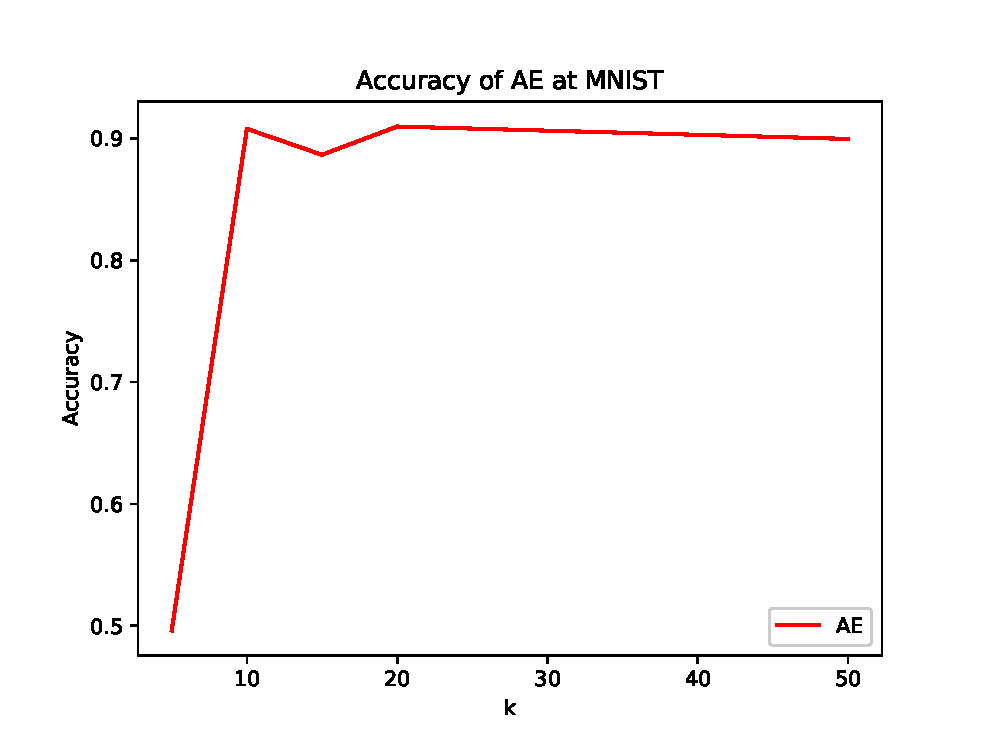
\includegraphics[width=0.45\linewidth]{Graphiken/MNIST_Accuracy_AE_k}}}
		\qquad
		\subfloat[ACC F-MNIST\label{fig:F-MNIST_ACC_kmeans_no_clusters}]{%			
		{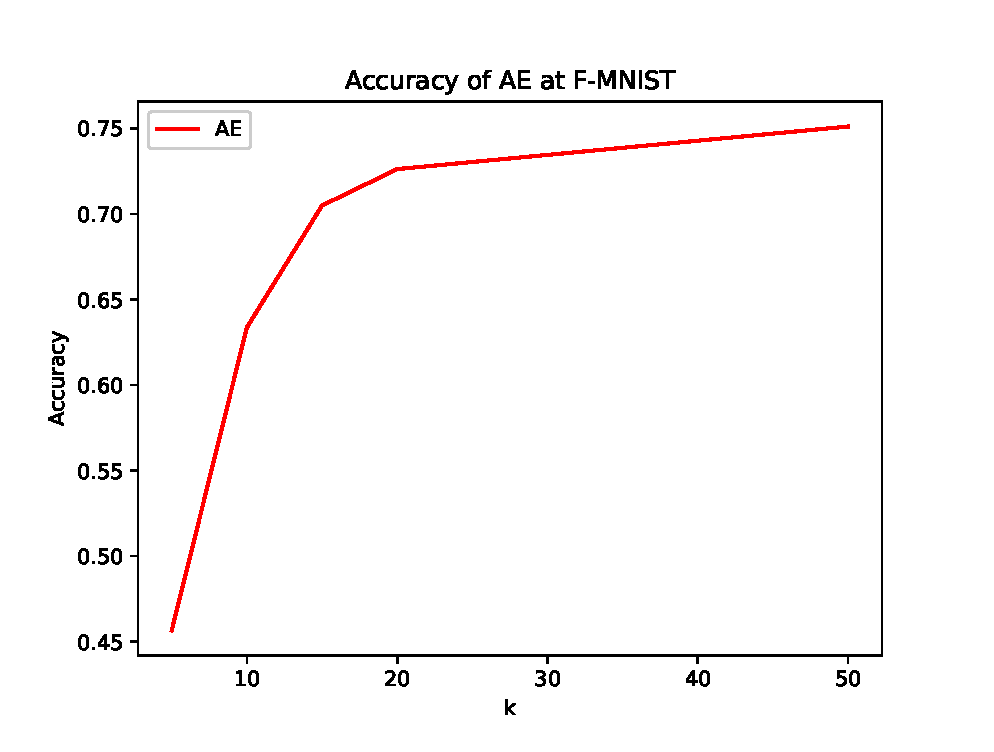
\includegraphics[width=0.45\linewidth]{Graphiken/F-MNIST_Accuracy_AE_k}}}
		\qquad
		\subfloat[ACC Imagenet-Dog\label{fig:Imagenet-Dog_ACC_kmeans_no_clusters}]{%			
		{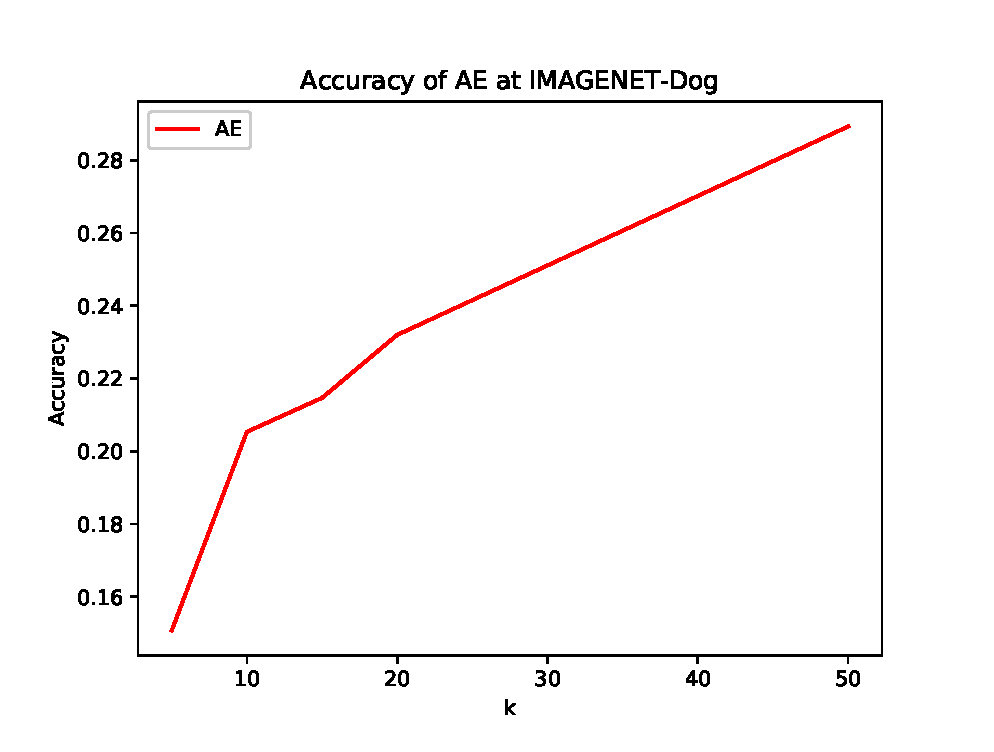
\includegraphics[width=0.45\linewidth]{Graphiken/IMAGENET-Dog_Accuracy_AE_k}}}
		\caption{Clustering Performance (ACC) for AE + K-means on different number of clusters $k$ for MNIST, F-MNIST and Imagenet-Dog}
		\label{fig:ClusterPerformance_kmeans_no_clusters}
	\end{figure}
The curves at F-MNIST (figure \ref{fig:F-MNIST_ACC_kmeans_no_clusters}) and Imagenet-Dog (figure \ref{fig:Imagenet-Dog_ACC_kmeans_no_clusters}) show the expected shape, with achieving higher accuracies with more number of clusters, as discussed beforehand. The curve at the MNIST dataset (figure \ref{fig:MNIST_ACC_kmeans_no_clusters}) shows a different behaviour. The curve achieves already a maximum with the number of clusters equals the original class number ($k=10$). One reason could be that the dataset can be partioned already well into $k=10$ different clusters which represent the original class numbers. By further dividing the clusters into more subclusters, the purity of the single clusters does not increase. This can be further proved by taking a look on the latent space of the AE after 50 training epochs with the help of the UMAP transformation of the $10$-dimensional latent space into $2$-d. This is visualized by figure \ref{fig:UMAP_2d_transform_MNIST_F-MNIST_AE}.
	 \begin{figure}[htb!]
		\centering	
		\subfloat[MNIST\label{fig:UMAP_2d_transform_MNIST_AE}]{%
		{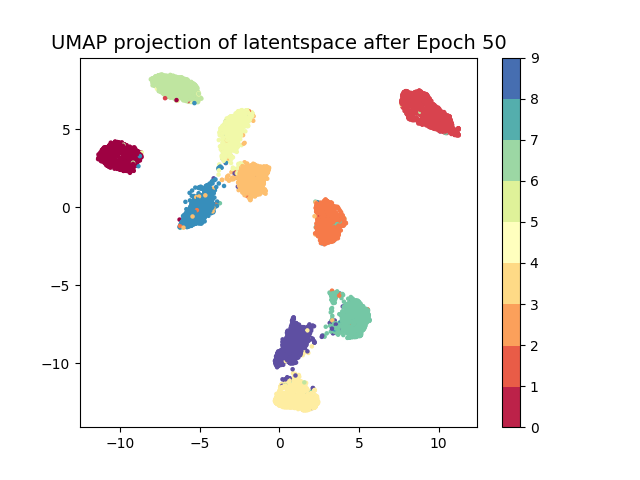
\includegraphics[width=0.45\linewidth]{Graphiken/UMAP_LatentSpace_AE_50epochs}}}
		\qquad
		\subfloat[F-MNIST\label{fig:UMAP_2d_transform_F-MNIST_AE}]{%
		{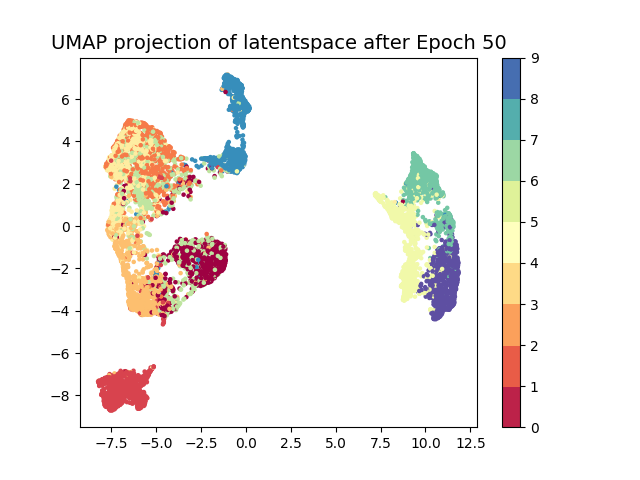
\includegraphics[width=0.45\linewidth]{Graphiken/UMAP_LatentSpace_AE_F-MNIST_50epochs}}}
		\caption{UMAP-transformed latent space of the AE after 50 epochs at MNIST and F-MNIST}
		\label{fig:UMAP_2d_transform_MNIST_F-MNIST_AE}
	\end{figure}
The figure shows, that the original classes can be seperated quite well by the latent representation of the AE at MNIST (figure \ref{fig:UMAP_2d_transform_MNIST_AE}). Further dividing the clusters into smaller clusters does not bring a benefit. When looking at the latent representations of the F-MNIST dataset (figure \ref{fig:UMAP_2d_transform_F-MNIST_AE}), it can be assumed, that further dividing clusters into smaller subclusters (increasing the number of cluster $k$) will increase the cluster accuracy. Additionally the impact of changing the number of clusters on the NMI is checked and visualized in figure \ref{fig:ClusterPerformance_NMI_kmeans_no_clusters}.
	 \begin{figure}[htb!]
		\centering
		\subfloat[MNIST\label{fig:MNIST_NMI_kmeans_no_clusters}]{%	
		{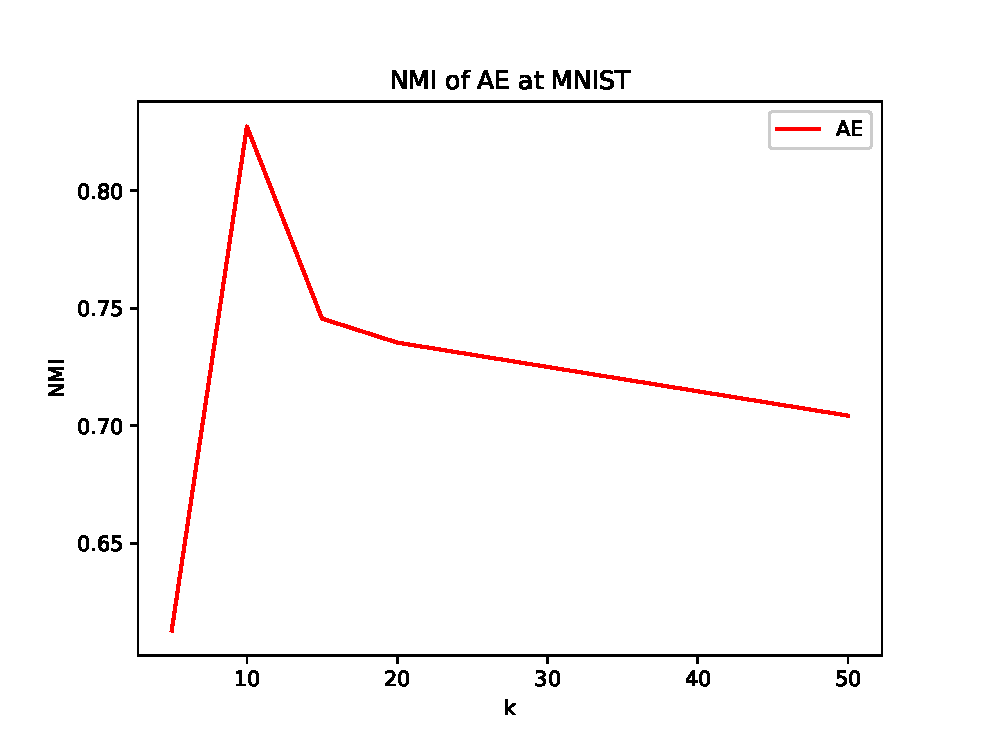
\includegraphics[width=0.45\linewidth]{Graphiken/MNIST_NMI_AE_k}}}
		\qquad
		\subfloat[F-MNIST\label{fig:F-MNIST_NMI_kmeans_no_clusters}]{%			
		{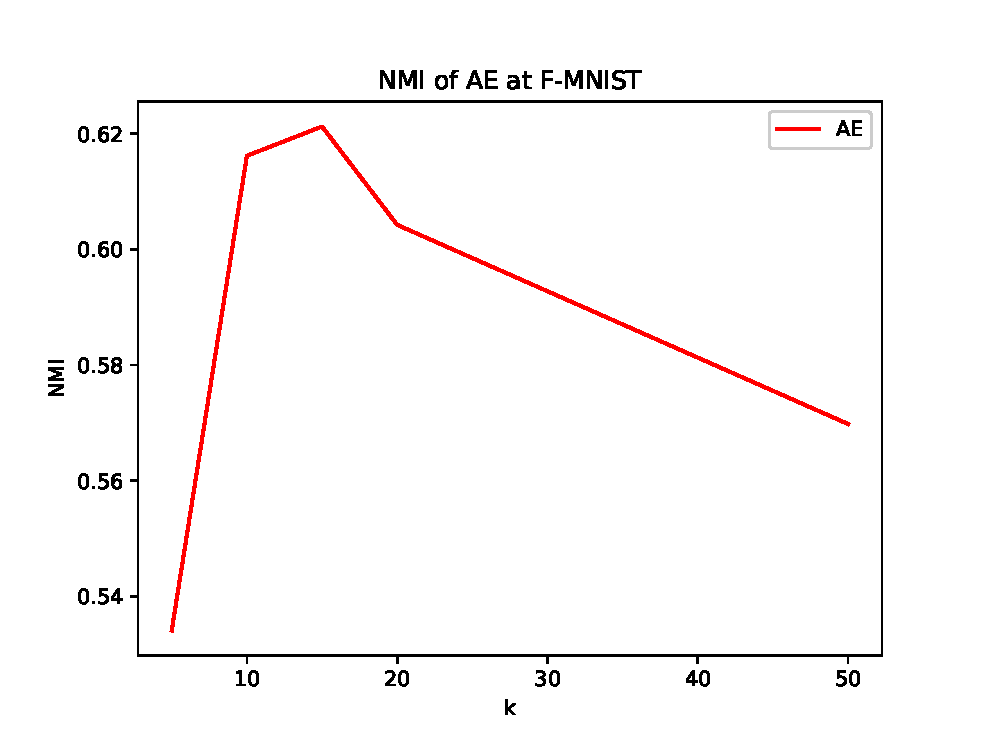
\includegraphics[width=0.45\linewidth]{Graphiken/F-MNIST_NMI_AE_k}}}
		\qquad
		\subfloat[Imagenet-Dog\label{fig:Imagenet-Dog_NMI_kmeans_no_clusters}]{%			
		{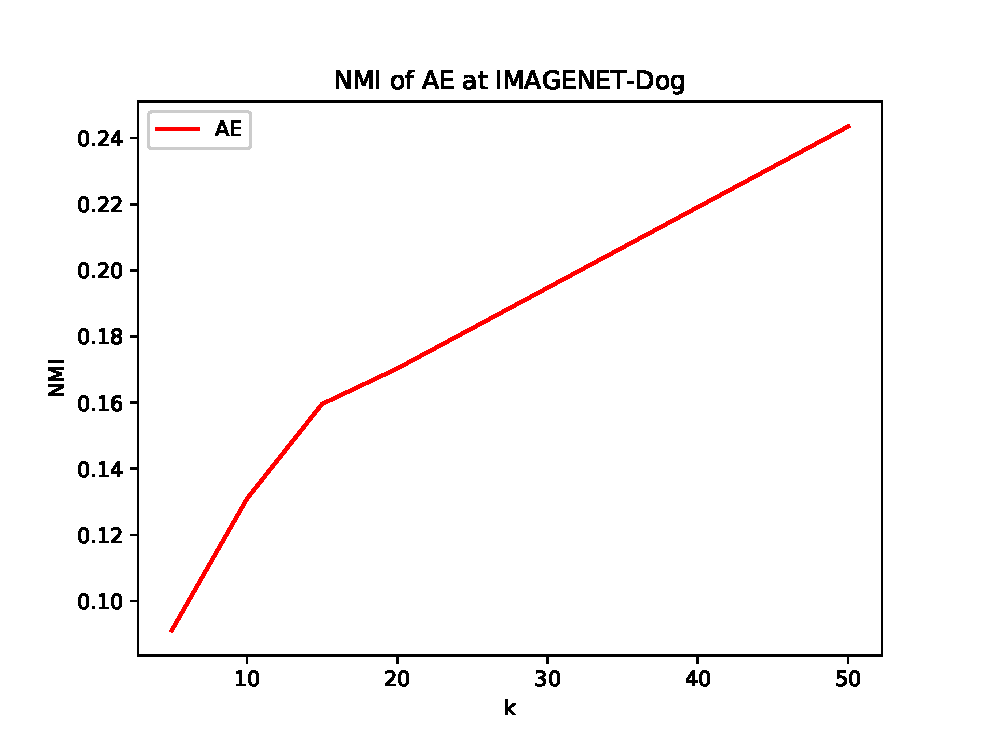
\includegraphics[width=0.45\linewidth]{Graphiken/IMAGENET-Dog_NMI_AE_k}}}
		\caption{Clustering Performance (NMI) for AE + K-means on different number of clusters $k$ for MNIST, F-MNIST and Imagenet-Dog}
		\label{fig:ClusterPerformance_NMI_kmeans_no_clusters}
	\end{figure}
The deviation of the NMI metric over $k$ can not be described generally for all datasets. Clearly, the better the distribution of the samples in the different clusters represents the true distribution, the higher the value of the NMI is. For MNIST (figure \ref{fig:MNIST_NMI_kmeans_no_clusters}) this optimum is obtained with a cluster number $k=10$, while for F-MNIST (\ref{fig:F-MNIST_NMI_kmeans_no_clusters}) the highest NMI value is reached at $k=15$. For Imagenet-Dog, the NMI value follows the behaviour of the clustering accuracy, increasing its value for higher number of clusters within the investigated range.\\
In addition, the impact of the batch size for the minibatch K-means algorithm, which is used in this work, is analysed. Therefore the batch size for the clustering task, $B_{clustering}$ is varied within the values $[64, 500, 1024, 2048]$. Due to memory limitation, a higher batch size is not feasible. So a classical K-means algorithm based on all data is not possible for every dataset (i.e. MNIST with 10000 test samples). The expectation is, that with higher batch sizes the performance should become more stable, since the K-means training steps become more stable (or vice-versa less noisy). With small batch sizes there is the risk, that the drawn samples in the batch does not represent the true distribution, so the cluster updates become biased towards the majority clusters inside a batch. The value $B_{clustering}=500$ can be seen as reference, since this value is used so far in this work. The number of clusters is fixed to the number of original classes in the dataset, other parameters stay the same as for the previous experiment. The resulting NMI values for the different batch sizes are shown in figure \ref{fig:ClusterPerformance_NMI_kmeans_eval_batch_size}.
	 \begin{figure}[htb!]
		\centering
		\subfloat[MNIST\label{fig:MNIST_NMI_kmeans_eval_batch_size}]{%	
		{\includegraphics[width=0.45\linewidth]{Graphiken/MNIST_NMI_AE_eval_batch_size}}}
		\qquad
		\subfloat[F-MNIST\label{fig:CIFAR-10_NMI_kmeans_eval_batch_size}]{%			
		{\includegraphics[width=0.45\linewidth]{Graphiken/CIFAR-10_NMI_AE_eval_batch_size}}}
		\caption{Clustering Performance (NMI) for AE + K-means on different cluster (eval) batch size for MNIST and CIFAR-10}
		\label{fig:ClusterPerformance_NMI_kmeans_eval_batch_size}
	\end{figure}
The expectation about the impact of the batch size on K-means clustering is fulfilled. With a higher batch size of the K-means minibatch algorithm, more stable (and even better) performance can be reached. This holds up to a certain value, where the minibatch K-means algorithm reaches a stable level of performance, with regard to small fluctuation still remaining since it remains a batched, and with that a noisy version of the original K-means algorithm. An additional remark is that for the Imagenet-10 and Imagenet-Dog datasets no minibatch version of K-means has to be used due to its small test datasets with $500$ and $750$ test samples, respectively.
\section{Final Results}
In this section, final results will be generated. Therefore the beforehand evaluated optimal hyperparameters per dataset and model are used to train the models with repetitions to generate also an estimate about the reproducibility of the results. First, the investigated hyperparameters will be introduced. These are used for the generation of the results per model and dataset. The hyperparameters are given in table \ref{tab:Hyperparametersettings_AE_b_AE}.
	\begin{table}[htb!]
    		\caption{Hyperparameter settings for different dataset for the AE/discriminative AE and VAE}
    		\label{tab:Hyperparametersettings_AE_b_AE}
    		\begin{tabular}{l|ccccc}
    			\toprule
        		Dataset $\backslash$ Hyperparameter & \multicolumn{2}{c}{$n_{latent}$} & \multicolumn{2}{c}{$B_{train}$} & $B_{cluster}$\\
        		& AE & VAE & AE & VAE & AE \& VAE\\
        		\midrule
        		MNIST & $10$ & $10$ & $64$ & $128$ & $1024$\\
        		F-MNIST & $10$ & $10$ & $64$ & $128$ & $2048$\\
        		CIFAR-10 & $20$ & $10$ & $64$ & $128$ & $2048$\\
        		CIFAR-100 & $32$ & $32$ & $64$ & $128$ & $2048$\\
        		Imagenet-10 & $128$ & $256$ & $64$ & $128$ & $500$\\
        		Imagenet-Dog & $256$ & $128$ & $64$ & $128$ & $500$\\
        		\bottomrule
    		\end{tabular}
    		\begin{tabular}{l|cccc}
    			\toprule
        		Dataset $\backslash$ Hyperparameter & \multicolumn{2}{c}{Learning Rate Schedule} & \multicolumn{2}{c}{$\gamma_0$}\\
        		& AE & VAE & AE & VAE\\
        		\midrule
        		MNIST & step decay & triangular & $0.1$ & $0.001$\\
        		F-MNIST & constant & triangular & $0.01$ & $0.01$\\
        		CIFAR-10 & triangular & triangular & $0.01$ & $0.01$\\
        		CIFAR-100 & triangular & triangular & $0.1$ & $0.01$\\
        		Imagenet-10 & exponential decay & triangular & $0.001$ & $0.001$\\
        		Imagenet-Dog & exponential decay & triangular & $0.01$ & $0.01$\\
        		\bottomrule
    		\end{tabular}
	\end{table}
Due to time restrictions, no separate hyperparameter tuning for the discriminative AE was possible. But based on the previous seen results it seems that the optimized hyperparameters for the AE also improve the clustering performance of the discriminative AE. Due to this, the discriminative AE will use the same hyperparameters as the AE, except for the training batch size $B_{train}$, which is set to $1000$ as already discussed. The Gumbel VAE show worse results with the obtained hyperparameters from the VAE. Due to this observation and time and computational restrictions, no further experiments with the Gumbel VAE were done. The later mentioned values are based on perviously achieved results with the Gumbel VAE. The other models listed are trained for $200$ epochs. Every 10th epoch clustering is executed. The best obtained clustering result based on the NMI is listed. For the AE, these procedure is repeated $5$ times per dataset. There the corresponding mean value is given with the standard deviation in brackets. For the discriminative AE and the VAE, $2$ runs per model and dataset is performed. The mean value is given and the corresponding deviation is written in the brackets. For all these models, the clustering is performed with K-means. Additionally, IDEC is performed based on the AE where possible, so where the latent size is equal to the given number of clusters. For the final result the number of clusters is set to the true number of classes. Clustering with IDEC is thus solely possible on MNIST and F-MNIST and is performed once with the best (in terms of NMI) AE model. The hyperparameters for IDEC are chosen as described in the original paper \cite{Guo17IDEC} and IDEC is trained for $50$ epochs. For a comparison, the Deep Adaptive Image Clustering (DAC) \cite{Chang17DAC} and original K-means is listed. DAC shows good clustering performance on different datasets and the performance metrics of this model are given for various datasets. Where the DAC is not listed for a dataset, no performance for this dataset is given. The best obtained mean value of the own models for each dataset and metric is marked in \textbf{bold}. The results are listed in table \ref{tab:ClusterPerformance_Models_final}.\\
	\begin{table}[htb!]
    		\caption{Clustering Performance of clustering models on different datasets with optimized hyperparameters}
    		\label{tab:ClusterPerformance_Models_final}
    		\centering
    		\begin{tabular}{l|ccc}
    			\toprule
    			\multicolumn{1}{c}{Dataset} & \multicolumn{3}{c}{MNIST}\\
        		\multicolumn{1}{c}{Metric} & ACC & NMI & ARI\\
        		\midrule
    			AE + K-means & $\mathbf{0.889}\ (0.043)$ & $0.815\ (0.020)$ & $0.796\ (0.044)$\\
        		discriminative AE + K-means & $0.780\ (0.021)$ & $0.716\ (0.018)$ & $0.613\ (0.015)$\\
        		VAE + K-means& $0.859\ (0.003)$ & $0.740\ (0.003)$ & $0.723\ (0.003)$\\
        		AE + IDEC & $0.872$ & $\mathbf{0.884}$ & $\mathbf{0.836}$\\
        		DAC & $0.978$ & $0.935$ & $0.949$\\
        		K-means & $0.626$ & $0.533$ & $0.415$\\
    		\end{tabular}
    		\begin{tabular}{l|ccc}
    			\toprule
    			\multicolumn{1}{c}{Dataset} & \multicolumn{3}{c}{F-MNIST}\\
        		\multicolumn{1}{c}{Metric} & ACC & NMI & ARI\\
        		\midrule
    			AE + K-means & $\mathbf{0.654}\ (0.023)$ & $\mathbf{0.645}\ (0.009)$ & $\mathbf{0.480}\ (0.018)$\\
        		discriminative AE + K-means & $0.621\ (0.044)$ & $0.609\ (0.019)$ & $0.446\ (0.032)$\\
        		VAE + K-means & $0.604\ (0.014)$ & $0.553\ (0.023)$ & $0.416\ (0.000)$\\
        		AE + IDEC & $0.589$ & $0.593$ & $0.418$\\
        		K-means & $0.612$ & $0.614$ & $0.428$\\
    		\end{tabular}
    		\begin{tabular}{l|ccc}
    			\toprule
    			\multicolumn{1}{c}{Dataset} & \multicolumn{3}{c}{CIFAR-10}\\
        		\multicolumn{1}{c}{Metric} & ACC & NMI & ARI\\
        		\midrule
    			AE + K-means & $\mathbf{0.270}\ (0.005)$ & $\mathbf{0.126}\ (0.004)$ & $0.070\ (0.002)$\\
        		discriminative AE + K-means & $0.256\ (0.008)$ & $0.109\ (0.006)$ & $0.061\ (0.005)$\\
        		VAE + K-means & $0.267\ (0.005)$ & $0.123\ (0.003)$ & $\mathbf{0.071}\ (0.001)$\\
        		DAC & $0.522$ & $0.396$ & $0.306$\\
        		K-means & $0.245$ & $0.102$ & $0.052$\\
    		\end{tabular}
    		\begin{tabular}{l|ccc}
    			\toprule
    			\multicolumn{1}{c}{Dataset} & \multicolumn{3}{c}{CIFAR-100}\\
        		\multicolumn{1}{c}{Metric} & ACC & NMI & ARI\\
        		\midrule
    			AE + K-means & $\mathbf{0.164}\ (0.003)$ & $\mathbf{0.102}\ (0.003)$ & $\mathbf{0.038}\ (0.001)$\\
        		discriminative AE + K-means& $0.097\ (0.005)$ & $0.042\ (0.001)$ & $0.010\ (0.003)$\\
        		VAE + K-means & $0.150\ (0.002)$ & $0.086\ (0.000)$ & $0.032\ (0.000)$\\
        		DAC & $0.238$ & $0.185$ & $0.088$\\
        		K-means & $0.145$ & $0.088$ & $0.031$\\
    		\end{tabular}
    		\begin{tabular}{l|ccc}
    			\toprule
    			\multicolumn{1}{c}{Dataset} & \multicolumn{3}{c}{Imagenet-10}\\
        		\multicolumn{1}{c}{Metric} & ACC & NMI & ARI\\
        		\midrule
    			AE + K-means & $0.260\ (0.008)$ & $0.125\ (0.005)$ & $0.055\ (0.003)$\\
        		discriminative AE + K-means& $0.235\ (0.001)$ & $0.113\ (0.002)$ & $0.043\ (0.001)$\\
        		VAE + K-means & $\mathbf{0.274}\ (0.000)$ & $0.128\ (0.003)$ & $\mathbf{0.057}\ (0.002)$\\
        		DAC & $0.527$ & $0.394$ & $0.302$\\
        		K-means & $0.256$ & $\mathbf{0.136}$ & $0.049$\\
    		\end{tabular}
    		\begin{tabular}{l|ccc}
    			\toprule
    			\multicolumn{1}{c}{Dataset} & \multicolumn{3}{c}{Imagenet-Dog}\\
        		\multicolumn{1}{c}{Metric} & ACC & NMI & ARI\\
        		\midrule
    			AE + K-means & $0.216\ (0.005)$ & $\mathbf{0.149}\ (0.004)$ & $\mathbf{0.044}\ (0.003)$\\
        		discriminative AE + K-means& $\mathbf{0.219}\ (0.006)$ & $\mathbf{0.149}\ (0.001)$ & $0.041\ (0.002)$\\
        		VAE + K-means & $0.199\ (0.009)$ & $0.129\ (0.001)$ & $0.037\ (0.001)$\\
        		DAC & $0.275$ & $0.219$ & $0.111$\\
        		K-means & $0.156$ & $0.089$ & $0.025$\\
        		\bottomrule
    		\end{tabular}
	\end{table}
	Overall, AE plus K-means can be seen as best clustering model within the here implemented and evaluated models. Nevertheless it has to be mentioned, that some optimization steps were only done for this model due to time restrictions. Comparing to the results, which are obtained at the beginning (table \ref{tab:ClusterACC_n_latent}) with the respective latent sizes of the AE, the performance could be improved significantly by optimizing the training of the AE (e.g. from $0.795$ clustering accuracy to $0.889$ on MNIST, or from $0.249$ to $0.270$ at CIFAR-10). Especially for the gray-scale images (MNIST, F-MNIST) the clustering of AE+K-means achieves good results with this model architecture, which is comparable to other more advanced architectures. But clearly, on more complicated datasets, i.e. CIFAR-100 or Imagenet-Dog, the performance of the model is limited. Also the hyperparameter optimization of the AE does not enable further clustering performance gains (i.e. from $0.162$ clustering performance to $0.164$ on CIFAR-100). It seems, that the chosen model complexity and thus the capability of the model architecture is too low to enable a good feature representation of the original images on the complex coloured image datasets, i.e. CIFAR-10 or CIFAR-100. This can be visualized by taking a look at the UMAP-transformed latent space for different epochs of the MNIST and CIFAR-10 dataset. The latent space after epoch 1 and 200 per dataset is visualized in figure \ref{fig:UMAP_AE_MNIST_CIFAR-10}.
	 \begin{figure}[htb!]
		\centering
		\subfloat[MNIST 1 epoch\label{fig:MNIST_UMAP_AE_1Epoch}]{%	
		{\includegraphics[width=0.45\linewidth]{Graphiken/UMAP_LatentSpace_AE_MNIST_1epochs}}}
		\qquad
		\subfloat[MNIST 200 epochs\label{fig:MNIST_UMAP_AE_200Epochs}]{%			
		{\includegraphics[width=0.45\linewidth]{Graphiken/UMAP_LatentSpace_AE_MNIST_200epochs}}}
		\qquad
		\subfloat[CIFAR-10 1 epoch\label{fig:CIFAR-10_UMAP_AE_1Epoch}]{%			
		{\includegraphics[width=0.45\linewidth]{Graphiken/UMAP_LatentSpace_AE_CIFAR-10_1epochs}}}
		\qquad
		\subfloat[CIFAR-10 200 epochs\label{fig:CIFAR-10_UMAP_AE_200Epochs}]{%			
		{\includegraphics[width=0.45\linewidth]{Graphiken/UMAP_LatentSpace_AE_CIFAR-10_200epochs}}}
		\caption{UMAP-transformed latent space of AE for MNIST (top) and CIFAR-10 (bottom) after 1 (left) and 200 epochs (right)}
		\label{fig:UMAP_AE_MNIST_CIFAR-10}
	\end{figure}
For the MNIST dataset, already after the first epoch some clusters can be separated clearly visually (e.g. dark and tight red in figure \ref{fig:MNIST_UMAP_AE_1Epoch}). Also the separated clusters represent already in principal purely the original classes. The cluster separation is increased further after 200 epochs, where the different clusters are well separated (figure \ref{fig:MNIST_UMAP_AE_200Epochs}). For the CIFAR-10 dataset, the two latent spaces after the first epoch (figure \ref{fig:CIFAR-10_UMAP_AE_1Epoch}) and after epoch 200 (\ref{fig:CIFAR-10_UMAP_AE_200Epochs}) look quite the same. The different clusters, and thus the latent representation for clustering is totally mixed and without the colouring of the true class labels, the representation could be seen as random. This is probably caused by the too low model capability. This means, that the model architecture, with the defined number of hidden layers and filters, is not capable to allow a meaningful feature reduction and representation from a $32x32x3$ images, so $3072$ features, to $20$ features (in the case of CIFAR-10 with an AE).\\
For a final large-scale investigation, the AE+K-means is trained on the entire Imagenet dataset with $1034908$ training images out of $1000$ classes and $50000$ test images \cite{imagenet_cvpr09} for $50$ epochs. The models are trained with a train batch size of $64$ and a clustering batch size of $2000$. One model, further denoted as \textit{model-1}, is trained with a latent space of $10$ and a constant learning rate of $0.1$. The other one, \textit{model-2}, has a latent space of $256$ and uses exponential decay as learning rate schedule with an initial learning rate of $0.01$. Figure \ref{fig:Visualization_Imagenet_Training} shows the training loss (figure \ref{fig:AE_Imagenet_TrainingLoss}) and the clustering accuracy over steps (figure \ref{fig:AE_Imagenet_ACC}). One steps denotes one update step, so passing one minibatch through the system and performing an corresponding parameter update.
\begin{figure}
	\centering
	\subfloat[Training loss\label{fig:AE_Imagenet_TrainingLoss}]{%
	\resizebox{0.45\linewidth}{!}{%
	\begin{tikzpicture}
		\begin{axis}[
			xmin = 0,
			style={thick},
			xlabel={num\_steps},
			ylabel={training loss}]
			\addplot[smooth, red] table[x=Step,y=Value, col sep = comma] {Graphiken/run_AE_IMAGENET_kmeans_2019-04-16_12-50_train_summaries-tag-loss.csv};
			\addplot[smooth, blue] table[x=Step,y=Value, col sep = comma] {Graphiken/run_AE_IMAGENET_kmeans_2019-04-17_13-48_train_summaries-tag-loss.csv};
			\legend{Model-1, Model-2}
		\end{axis}
	\end{tikzpicture}}}
	\qquad
	\subfloat[Clustering Accuracy\label{fig:AE_Imagenet_ACC}]{%	
	\resizebox{0.45\linewidth}{!}{%
	\begin{tikzpicture}
		\begin{axis}[
			xmin = 0,
			ymin=0,
			ymax=0.03,
			style={thick},
			xlabel={num\_steps},
			ylabel={Clustering Accuracy}]
			\addplot[smooth, red] table[x=Step,y=Value, col sep = comma] {Graphiken/run_AE_IMAGENET_kmeans_2019-04-16_12-50_eval_summaries-tag-Accuracy.csv};
			\addplot[smooth, blue] table[x=Step,y=Value, col sep = comma] {Graphiken/run_AE_IMAGENET_kmeans_2019-04-17_13-48_eval_summaries-tag-Accuracy.csv};
			\legend{Model-1, Model-2}
		\end{axis}
	\end{tikzpicture}}}
	\caption{Training loss (left) and Clustering Accuracy (right) on Imagenet over steps}
	\label{fig:Visualization_Imagenet_Training}
\end{figure}
As already discussed earlier in this work and seen again here, a smaller latent space (\textit{model-1}) leads on the one hand to higher reconstruction loss, but on the other hand it allows better clustering. The best obtained values for training error and the introduced cluster metrics (ACC, NMI, ARI) are summarized in table \ref{tab:ClusterPerformance_AE_Imagenet} for the two models. 
	\begin{table}[htb!]
    		\caption{Clustering Performance of AE + K-means on complete Imagenet with different latent spaces and training procedures}
    		\label{tab:ClusterPerformance_AE_Imagenet}
    		\centering
    		\begin{tabular}{l|cccc}
    			\toprule
    			\multicolumn{1}{c}{Dataset} & \multicolumn{4}{c}{Imagenet}\\
        		\multicolumn{1}{c}{Metric} & Training Error & ACC & NMI & ARI\\
        		\midrule
    			Model-1 & $0.027$ & $0.018$ & $0.259$ & $0.002$\\
    			Model-2 & $0.007$ & $0.012$ & $0.153$ & $0.002$\\
        		\bottomrule
    		\end{tabular}
	\end{table}
The performance is, as expected, not good, but it has to be set into the relation of the dataset. First, it has to be to mentioned, that the clustering training for K-means is done with a batch size of $2000$, which in this case with $1000$ classes means that the training is not optimal. As observed earlier, the batch size should be much higher than the number of clusters $k$. This could not be fullfilled due to memory restrictions. Finally, a clustering accuracy of $1.8\%$ is a factor $18$ higher than random guessing, which would result in a clustering accuracy of $0.1\%$. So the clustering is encoding some similar images correctly to a similar latent space representation. However, it can be seen in figure \ref{fig:AE_Imagenet_ACC} that no significant improvement with respect to clustering can be achieved over the training steps, which means that the model is not able to learn more relevant feature representations than learned in the first epochs.\\
The other two models, the discriminative AE and the VAE show general worse clustering performance than the AE. For the VAE, a reason can be, that the VAE as a generative model represents the data in a more continuous latent space. From clustering perspective, this is not an optimal property. This property is visible in figure \ref{fig:UMAP_AE_b_AE_VAE_MNIST}, which shows the latent spaces of the three models at MNIST after 200 epochs.
	 \begin{figure}[htb!]
		\centering
		\subfloat[AE\label{fig:MNIST_UMAP_AE_200Epochs}]{%	
		{\includegraphics[width=0.45\linewidth]{Graphiken/UMAP_LatentSpace_AE_MNIST_200epochs}}}
		\qquad
		\subfloat[discriminative AE\label{fig:MNIST_UMAP_b_AE_200Epochs}]{%			
		{\includegraphics[width=0.45\linewidth]{Graphiken/UMAP_LatentSpace_b_AE_MNIST_200epochs}}}
		\qquad
		\subfloat[VAE\label{fig:MNIST_UMAP_VAE_200Epochs}]{%			
		{\includegraphics[width=0.45\linewidth]{Graphiken/UMAP_LatentSpace_VAE_MNIST_200epochs}}}
		\caption{UMAP-transformed latent space of AE, discriminative AE and VAE for MNIST after 200 epochs}
		\label{fig:UMAP_AE_b_AE_VAE_MNIST}
	\end{figure}
	It can be seen that the latent space of the VAE (figure \ref{fig:MNIST_UMAP_VAE_200Epochs}) is more continuous, so the latent representations are not that well separated as for the AE (figure \ref{fig:MNIST_UMAP_AE_200Epochs}) or the discriminative AE (figure \ref{fig:MNIST_UMAP_b_AE_200Epochs}). For the discriminative AE, the additional introduced objective, that similar original image are encoded into the same area in the latent space, can also be seen. This is not necessarily an advantage for MNIST, because e.g. the images of classes $3$, $6$ and $9$ are encoded into a similar region (the three clusters in the middle right with colours orange, light green and blue) because there are obviously similar original images between the classes for handwritten digits. Therefore, the choice of anchor pairs and the number of them is crucial for this model, but this was not evaluated in detail within this work.
\chapter{Summary and Outlook}
In this work, current state-of-the-art clustering algorithms are evaluated. The implemented, optimized and evaluated models consist of two parts. First an AE-based feature/dimensionality reduction needs to be performed and then, based on the latent representations, clustering can be performed. Four models to reduce/extract the features are introduced which were evaluated with respect to clustering on six different datasets. One standard AE and one classical VAE were used, and additionally an adaptation of the two models, with the discriminative AE and the Gumbel VAE. All models are based on the same general architecture regarding number of hidden layers or filter sizes. For these models, a large-scale evaluation on the different datasets was performed. First, the hyperparameter of the models were fixed.\\
Therefore an optimal size of the latent space for clustering was needed. It could be shown clearly, that the clustering and the reconstruction task are mostly conflictive to each other for AE-based models. This means, that with smaller latent spaces, the clustering performance increases, but the reconstruction capability reduces. The optimum size of the latent space directly depends on the dataset, e.g. for MNIST dataset the relevant features can be reduced into a very small dimensional space (e.g. $10$), while for more complicated images (e.g. Imagenet-10) the relevant features can't be compressed into a that small latent space. For high latent spaces, the AE reaches a stable minima regarding clustering performance, while the VAE approaches to a NMI of $0$ for high values.\\
For the discriminative AE, the hyperparameters for regularization of the reconstruction loss $\lambda_r$ and for the uncertainty of the anchor pairs $\alpha$ are optimized by a grid search. Based on the evaluated NMI-values on the different dataset, the hyperparameters are set to $\lambda_r=1$ and $\alpha=0.5$.\\
The Gumbel VAE has as a separate hyperparameter the temperature $\tau$ of the Gumbel distribution. Nevertheless, the value of $\tau$ is directly influencing the latent space, that's why for a better understanding different latent spaces were again evaluated. The two hyperparameters are evaluated with a grid search and the respective NMI-values on different datasets. Based on these results, the optimal hyperparameters for the Gumbel VAE would be $n_{latent}=64$ and $\tau=10$, so a quite uniform distributed latent space. Nevertheless, for comparability the same latent space size as for the standard VAE was used with $\tau=10$.\\
With the \textit{fixed} models the training procedure of the feature reduction models was optimized by adapting specific training-related hyperparameters. First, the impact of the training batch size in combination with different constant learning rates was evaluated. Therefore a grid search in defined ranges was performed. In general, the clustering performance increases with smaller batch sizes for the AE, so the training batch size was set to $64$ based on the evaluated experiments. For the VAE, the optimum training batch size regarding clustering performance was found to be $128$ in these experiments. The optimal learning rate depends on the dataset. Due to time restrictions, these evaluations couldn't be performed for the remaining two models, so the obtained parameter values from AE and VAE are used for the discriminative AE and the Gumbel VAE. With these adaptations, the clustering performance could be already increased significantly, e.g. from $80\%$ to $89\%$ clustering accuracy with the AE+K-means at MNIST. For the more complex datasets, e.g. CIFAR-100, the performance improves not that much, or even no performance improvement could be achieved (e.g. at CIFAR-100).\\
Further additional learning rate schedules (step decay, exponential decay and triangular learning rate schedule) are evaluated with different initial learning rates. For the AE, the schedule and initial learning which achieves the best clustering performances varies from dataset to dataset. For the VAE, the triangular learning rate schedule achieves the best clustering performance values of all datasets. The optimum initial learning rate varies there, too. With these adaptations, the clustering performance could further be increased, e.g. to $91\%$ on MNIST with the AE+K-means.\\
Based on these optimal learning rate schedules, another modification to the learning rate scheduling, the linear warmup, was evaluated. For the different schedules, the effect of a linear warmup to the clustering performance was checked. Overall, the performance did not increase further. For some combinations (e.g. step decay with AE at Imagenet-10) the performance could be slightly improved. But in the most cases, the clustering performance stays on the same level as it was without linear warmup or even became worse (e.g. step decay with AE at MNIST). Therefore, the linear warmup was not further used.\\
After the training procedure was optimized for the feature reduction models, different parameter settings for the training of the K-means, and thus the clustering robustness of the K-means, were evaluated. Therefore, the effect of different number of clusters was evaluated. As expected, the clustering accuracy (also denoted as purity) increased with more clusters at all datasets, out of for MNIST, where it stays quasi stable for $k\geq10$. Probably the clusters are already that well separated, that further dividing the clusters can not increase the cluster purity.\\
Furthermore, the clustering performance for different clustering batch sizes was evaluated. In this work, due to memory restrictions, a minibatch K-means was used, and thus the expectation is, that the clustering batch size influence the training procedure of the K-means, which could be proved. In general, the clustering performance becomes more stable for higher batch sizes, because the sample distribution approaches the true distribution of the samples.\\
With these adapted and optimized hyperparameters, a final evaluation was done. For the gray-scale datasets (MNIST and F-MNIST) the achieved performance was comparable to current more complicated clustering algorithms. For the coloured datasets (e.g. CIFAR-100) the performance could not be increased that much or even no further performance improvement could be achieved. The chosen model complexity of the feature reduction seems to be too low for reducing relevant features for the clustering tasks out of these images. In this work it could be proved, that by optimizing the training procedure of an AE, the final clustering performance can be increased significantly. Therefore, a possible next step would be to evaluate a more complex AE architecture with respect to hidden layers or other model parameters (number of filters) and optimize the model for the more challenging datasets. There exist also a lot of popular methods in the deep learning area, which could be also interesting for these tasks. As an example, residual connections could be used to further accelerate the convergence of the AE training, and thus enable more complex architectures. In addition, the choice of the loss function seems to have optimization potential. The currently most used loss function for an AE is the Mean Squared Error (MSE), which actually gives a pixelwise error value. However, especially for coloured (more complex) datasets, this does not seem to be reasonable, because there is a high potential, that the AE gives e.g. more attention to a blue background than on the small, but relevant object (e.g. an air plane). Possible loss functions which measure image similarity based on more relevant attributes (i.e. edges) are the structural similarity metric (SSIM \cite{Wang04SSIM}) or the multi-scale SSIM (MS-SSIM \cite{Wang03MSSSIM}). These adaptations could also be used directly for finding the so called \textit{anchor pairs} for the discriminative AE. Instead of using the pixel-based similarities, the more realistic similarity metrics could be used to find these pairs. For the VAE, it could be interesting to force the latent space to model latent representations not in one high-dimensional gaussian distribution, but on $k$ different gaussian distributions. Then a direct clustering with a Maximum-Likelihood estimator could be possible on the latent representation, when having $k$ different gaussian (target) distributions. This could also be directly used for the Gumbel VAE, with $k$ Gumbel Softmax distributions and every distribution modelling one cluster out of $k$. For the Gumbel VAE, a separate hyperparameter tuning could be useful. The main idea, becoming more discrete, or even real discrete, latent representations, is from a theoretical point of view helpful in terms of clustering, because this forces the encoder to separate the samples already when encoding them into the latent space. Nevertheless, in this work this separate optimization could not be done, and the used hyperparameter settings obtained for the VAE seems to be no reasonable choice, since those reduced the clustering performance of the Gumbel VAE.\\
Overall, AE based feature reduction models show the possibility to encode original images in cluster-friendly latent spaces.

	% -------------------> end writing here <------------------------
	% *****************************************************************
	\ifthenelse{\equal{\doclang}{german}}{
		\bibliographystyle{IEEEtran_ISSger}
	}{
		\bibliographystyle{IEEEtran_ISS}
	}
	\bibliography{refs}
	
	% *****************************************************************
	%% Additional page with Declaration ("Eidesstattliche Erklrung");
	%% completed automatically
	\begin{titlepage}
		\vfill
		\LARGE \ifthenelse{\equal{\doclang}{german}}{\textbf{Erkl\"arung}}{\textbf{Declaration}}
		\vfill
		
		\ifthenelse{\equal{\doclang}{german}}{
			Hiermit erkl\"are ich, dass ich diese Arbeit selbstst\"andig verfasst und keine anderen als die angegebenen
			Quellen und Hilfsmittel benutzt habe.
		}
		{
			Herewith, we declare that we have developed and written the enclosed thesis entirely by ourself and that I have not used sources or means except those declared.
		}
		
		\vspace{1cm}
		
		\ifthenelse{\equal{\doclang}{german}}{
			Die Arbeit wurde bisher keiner anderen Pr\"ufungsbeh\"orde vorgelegt und auch noch nicht ver\"offentlicht.
		}
		{
			This thesis has not been submitted to any other authority to achieve an academic grading and has not been published elsewhere.
		}
		
		\vfill
		
		
		Stuttgart, \signagedate
		\hfill
		\begin{tabular}{l}
			\hline
			\student
		\end{tabular}
	\end{titlepage}
	
	
	
\end{document}
